\documentclass[a4paper]{article}
\usepackage{graphicx}
\usepackage{geometry}
\usepackage{pdfpages}
\usepackage{calc}
\usepackage{anyfontsize}
\usepackage{xcolor}
\definecolor{COLV}{RGB}{148,0,0}
\definecolor{COLT}{RGB}{20,20,20}
\usepackage{adforn}
\usepackage[cmintegrals,cmbraces]{newtxmath}
\usepackage{ebgaramond-maths}
\usepackage{trajan}
\usepackage[T1]{fontenc}
\pagestyle{empty}
\newcommand\twocolouri{\hspace*{0pt}\raisebox{\heightof{\i}+0.2ex}{\rlap{\textcolor{COLV}{.}}}\i}
\newcommand\blackcolouri{\hspace*{0pt}\raisebox{\heightof{\i}+0.2ex}{\rlap{\textcolor{COLT}{.}}}\i}
\newlength{\titlew}\setlength{\titlew}{\widthof{\fontsize{50pt}{20pt}\selectfont\color{COLV}Portfolio}}
\setlength{\parindent}{0pt}
\newcommand{\titlesize}{\fontsize{30pt}{30pt}\selectfont}
\newcommand{\fleuronsize}[1]{\scalebox{4}{#1}}
\newcommand{\titlefleuron}[2]{\clearpage%
    \begin{center}\titlesize
        #1\\
        \vfill
        \textcolor{COLV}{\fleuronsize{#2}}
        \vfill
        \null
    \end{center}\clearpage
}
\newcommand{\titlenofleuron}[2]{\clearpage%
    \begin{center}\titlesize
        #1\\
        \vfill
        #2
        \vfill
        \null
    \end{center}\clearpage
}
\newcommand{\simpletitle}[1]{\clearpage%
    \begin{center}\titlesize
        #1\\
    \end{center}
}
\newcommand{\centerfleuron}[1]{\vfill\begin{center}\color{COLV}\fleuronsize{#1}\end{center}\vfill\null}
\newcommand{\collaboration}[2]{%
    \vfill
    \begin{minipage}{0.6\linewidth}\raggedright\Large#1\end{minipage}%
    \begin{minipage}{0.4\linewidth}\raggedleft\includegraphics[width=\linewidth]{./images/#2}\end{minipage}
}
\newcommand{\pcollaboration}[1]{{\LARGE #1}\\\strut\\}
\newcommand{\feedback}[2][\large]{%
    \begin{minipage}{\linewidth}\tt#1
    ``#2''
    \end{minipage}\\[1.5\baselineskip]
}
\begin{document}
%%%%%%%%%%%%%%%%%%%%%%%%%%%%%%%%%%%%%%%%%%%%%%%%%%%%%%%%%%%%%%%%%%%%%
% Title page
%%%%%%%%%%%%%%%%%%%%%%%%%%%%%%%%%%%%%%%%%%%%%%%%%%%%%%%%%%%%%%%%%%%%%
    \null
    \vfill
    \begin{center}
        {\fontsize{50pt}{20pt}\selectfont\color{COLV}Portfol\blackcolouri o}\\
        \strut\\
        \resizebox{\titlew}{!}{\color{COLT}El\twocolouri o \textit{A}\kern-1pt\textcolor{COLV}{.} Far\twocolouri na}
    \end{center}
    \vfill
    \begin{center}
    
\includegraphics[width=0.3\linewidth]{./TikZimages/logoofficial.pdf}\\
    {\small\trjnfamily \strut\\ CARERE DEBET OMNI VITIO\\ QUI IN ALTERUM DICERE PARATUS EST}
    \end{center}

%%%%%%%%%%%%%%%%%%%%%%%%%%%%%%%%%%%%%%%%%%%%%%%%%%%%%%%%%%%%%%%%%%%%%
% Colophon
%%%%%%%%%%%%%%%%%%%%%%%%%%%%%%%%%%%%%%%%%%%%%%%%%%%%%%%%%%%%%%%%%%%%%
    \clearpage
    \begin{flushright}
        \textit{\huge Al \LaTeX}
    \end{flushright}
        \vfill
    \begin{center}
        \rotatebox{270}{\scalebox{25}{\color{COLV},}}
    \end{center}
        \vfill
    \strut\hfill\begin{tabular}{@{}r@{}}
        \Large\itshape Elio is stubborn and brilliant.\\
        \Large\itshape Starting to work with him is one of the best things that has ever happened to me.\\
        \strut\\
        \Large Nils Rudi\\
        \Large Professor at Yale
    \end{tabular}
        \vfill
    \begin{flushright}
        \huge
        Portfolio\\
        Elio A. Farina\\
        \LARGE
        \strut\\
        %personal email: elio.farina@gmail.com\\
        %Overleaf account: elio.farina@gmail.com\\
        %GitHub: https://github.com/elioa/\\
        %BitBucket: https://bitbucket.org/elioa/\\
        %Personal WebSite: badroomtales.me\\
        \strut\\
        100\% \LaTeXe\ made
    \end{flushright}
\clearpage
\begingroup\LARGE\raggedright\setlength{\parskip}{\baselineskip}
Hemingway once said,\\ ``There is nothing to writing. All you do is sit down at a typewriter and bleed.''

My take is that there is everything to \LaTeX{}: all I have to do is sit down at my computer and make the magic happen.

My name is Elio A. Farina, and I’m a \LaTeX{} coder.

I met \LaTeX{} in 2000, and it was love at first sight! I use \LaTeX{} for everything in my life when I have to deal with typesetting and design, and since 2015, coding in \LaTeX{} has been my only job. I’ve collaborated and I’m still collaborating with various individuals and organisations around the world to turn their dreams into realities. Well, at least their \LaTeX{} dreams!

\LaTeX{} is not just for typesetting your dissertation because your advisor said so. And for sure, it doesn’t have to be painful and you don’t need to bleed, as Hemingway suggested. It is about coding, and most of my jobs involve drawing images using TikZ, creative problem solving and \LaTeX{} integration with several other programming experiences. And macro naming. Most of my energy goes into naming.

If you need \LaTeX{} help for whatever your reasons are, I’m here for you!
\endgroup
\clearpage
%%%%%%%%%%%%%%%%%%%%%%%%%%%%%%%%%%%%%%%%%%%%%%%%%%%%%%%%%%%%%%%%%%%%%
% Page layout
%%%%%%%%%%%%%%%%%%%%%%%%%%%%%%%%%%%%%%%%%%%%%%%%%%%%%%%%%%%%%%%%%%%%%
    \titlefleuron{Page layout}{\adfhangingflatleafleft}

    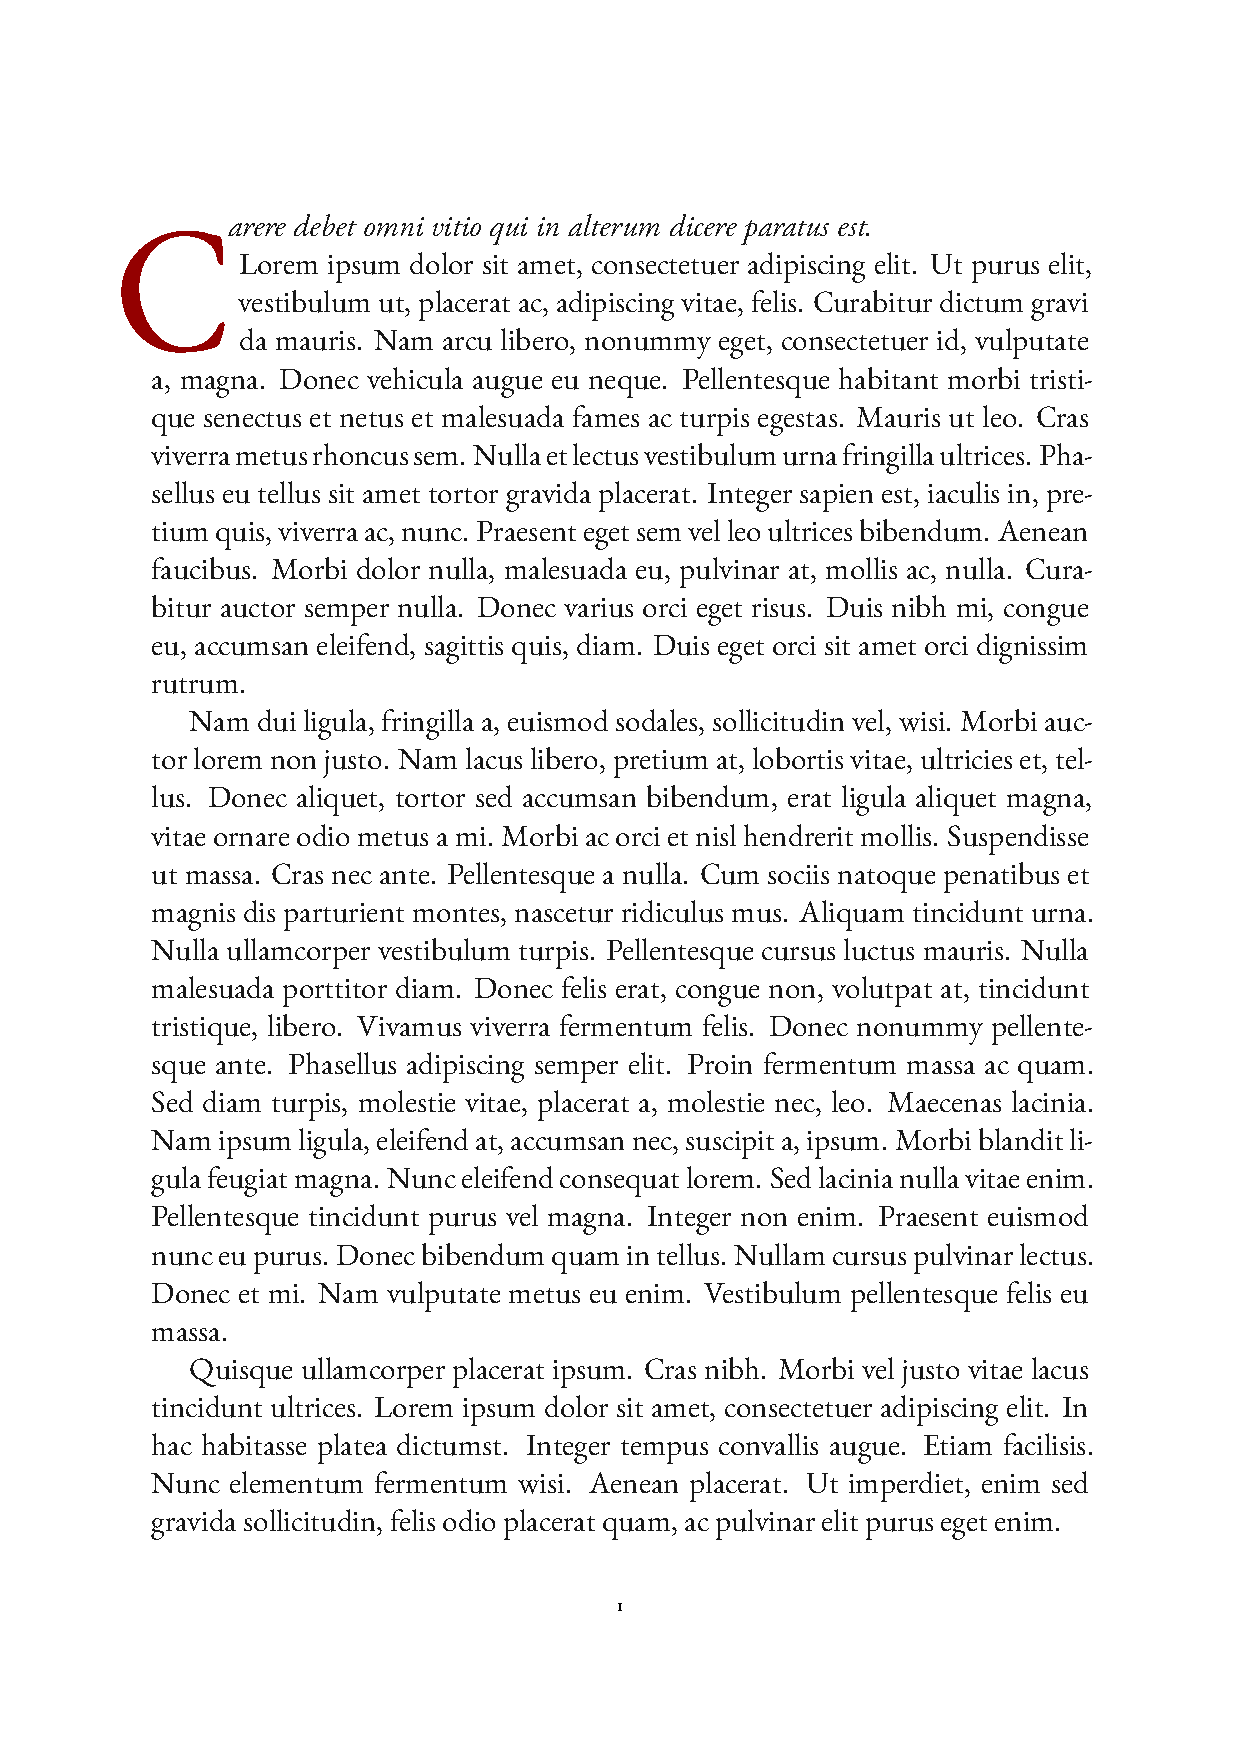
\includepdf{./FullPages/Layout5.pdf}
    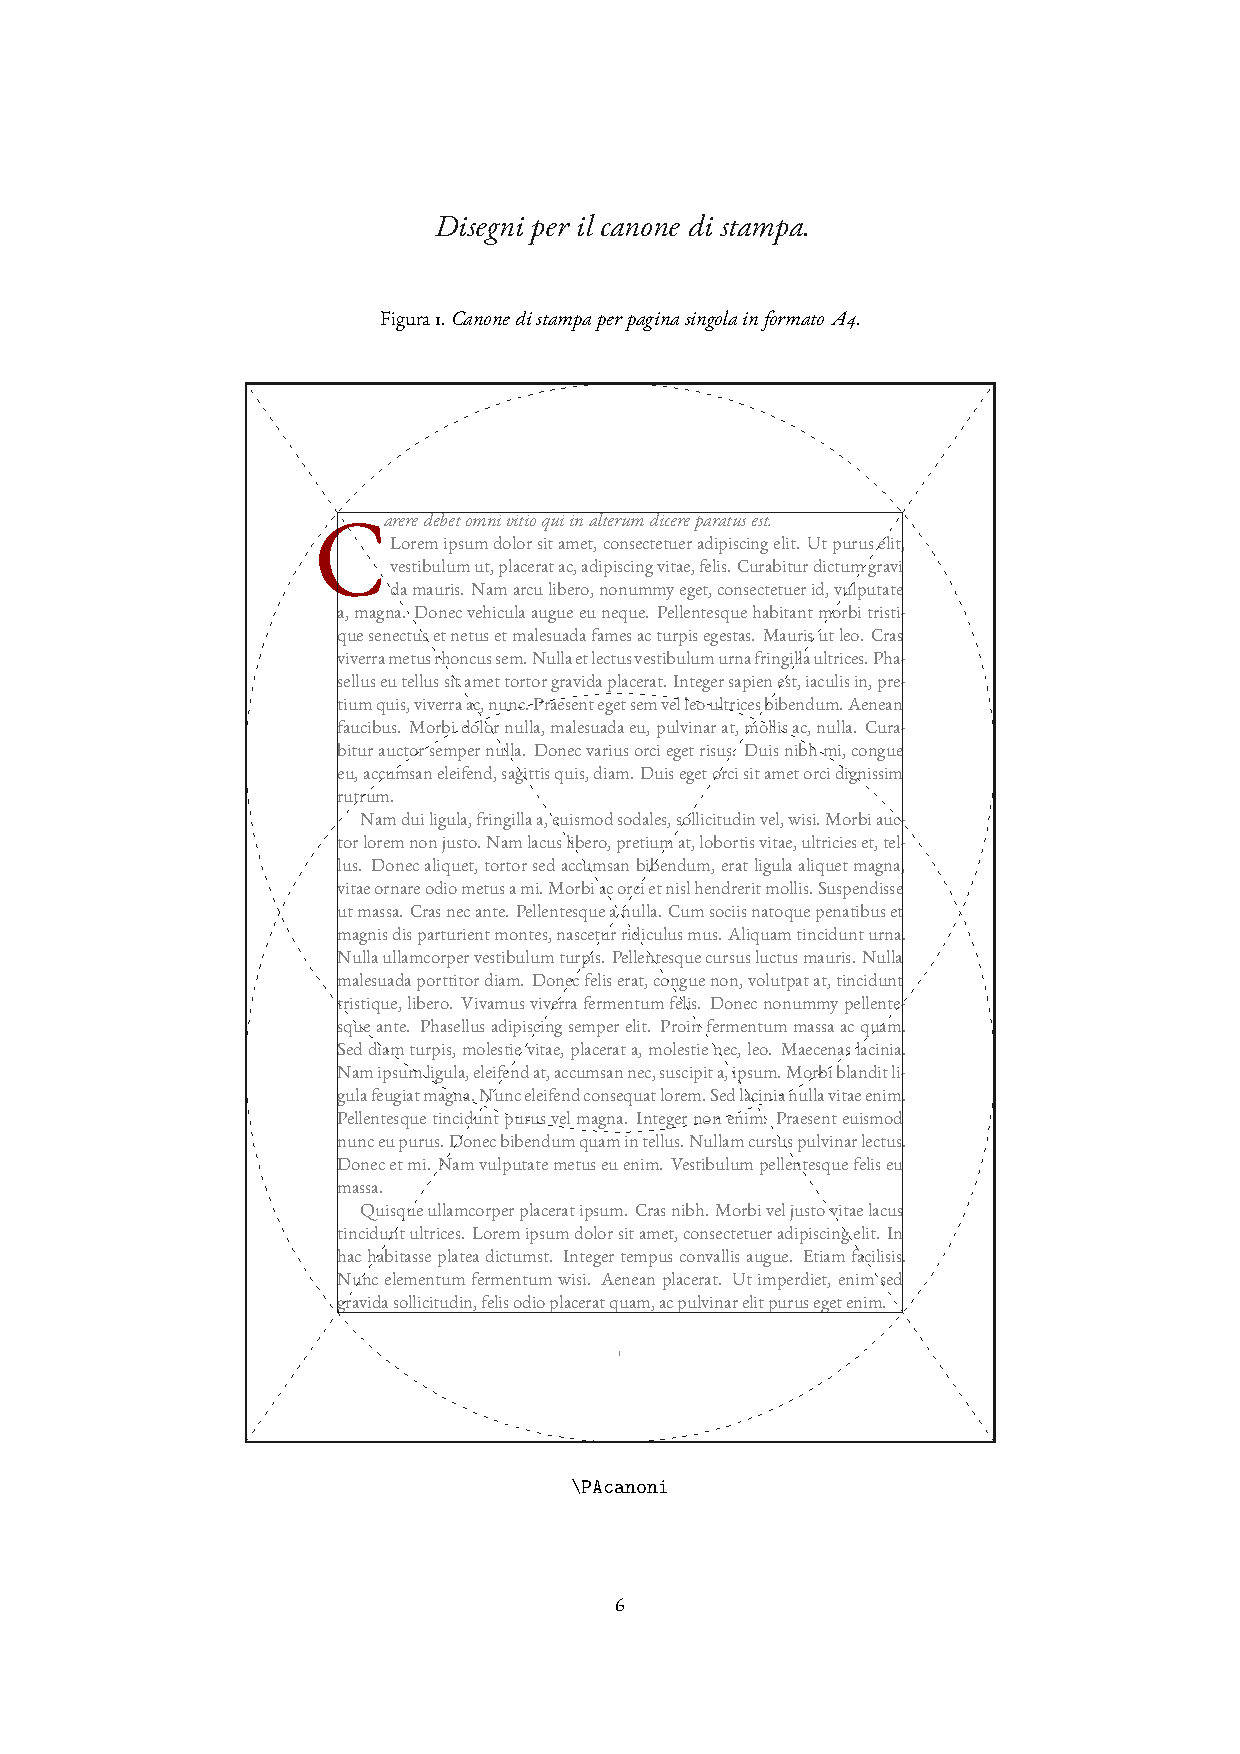
\includepdf{./FullPages/Layout6.pdf}
    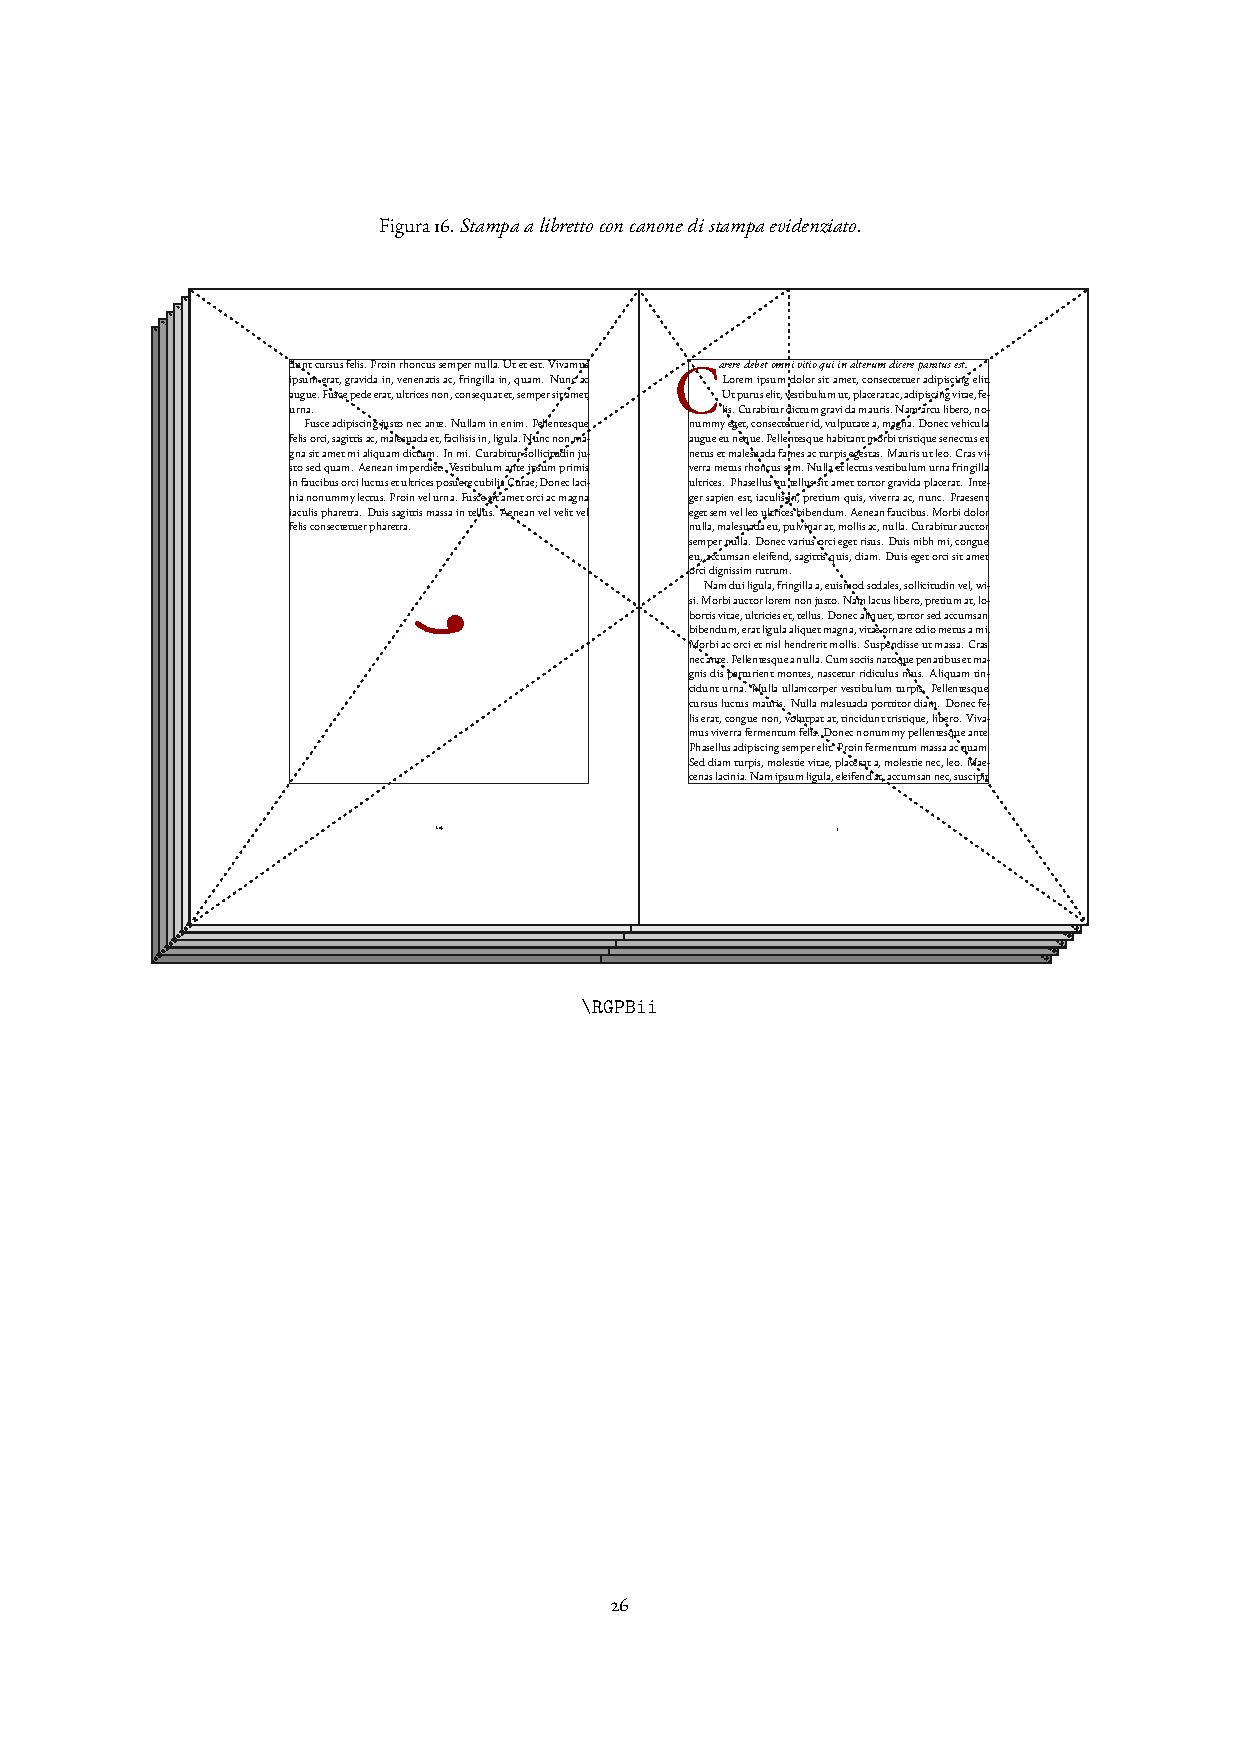
\includepdf{./FullPages/Layout7.pdf}
    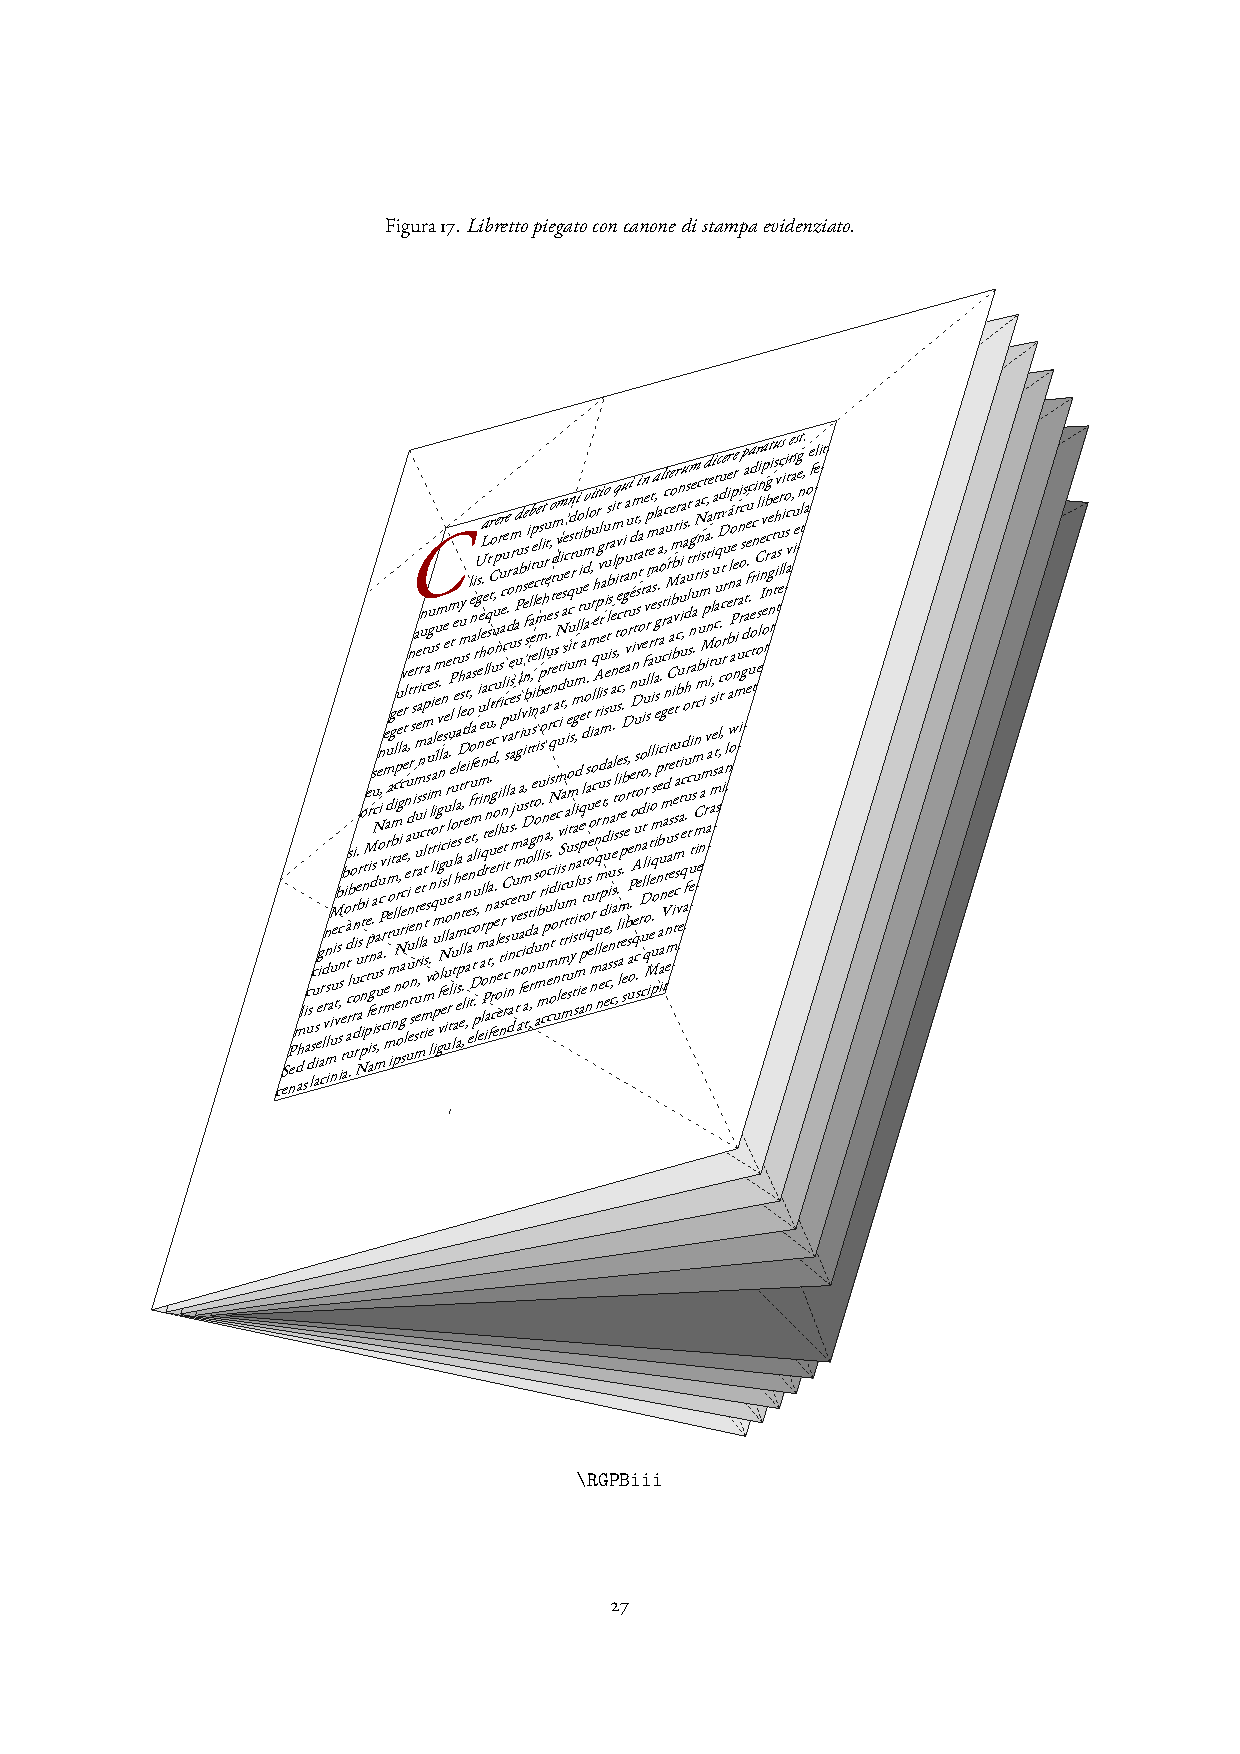
\includepdf{./FullPages/Layout8.pdf}
    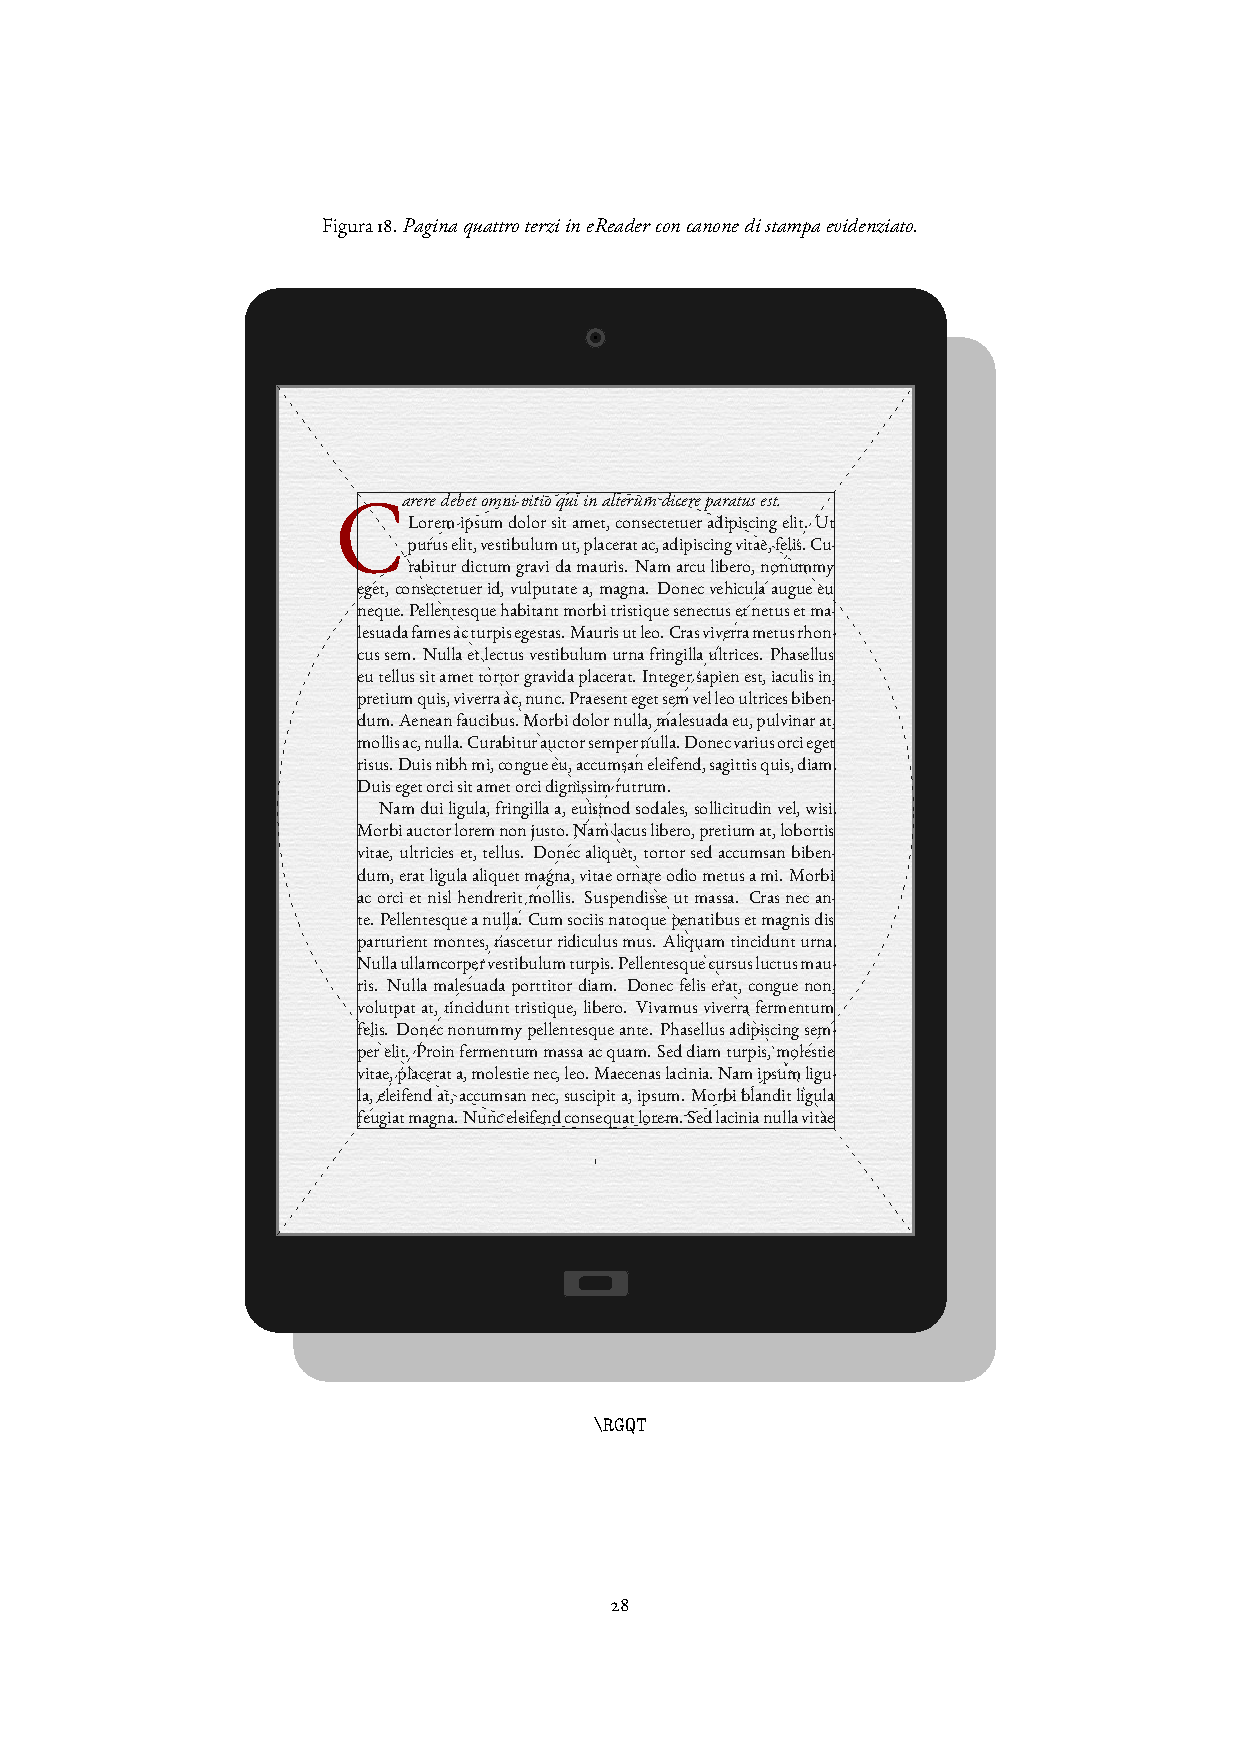
\includepdf{./FullPages/Layout9.pdf}
    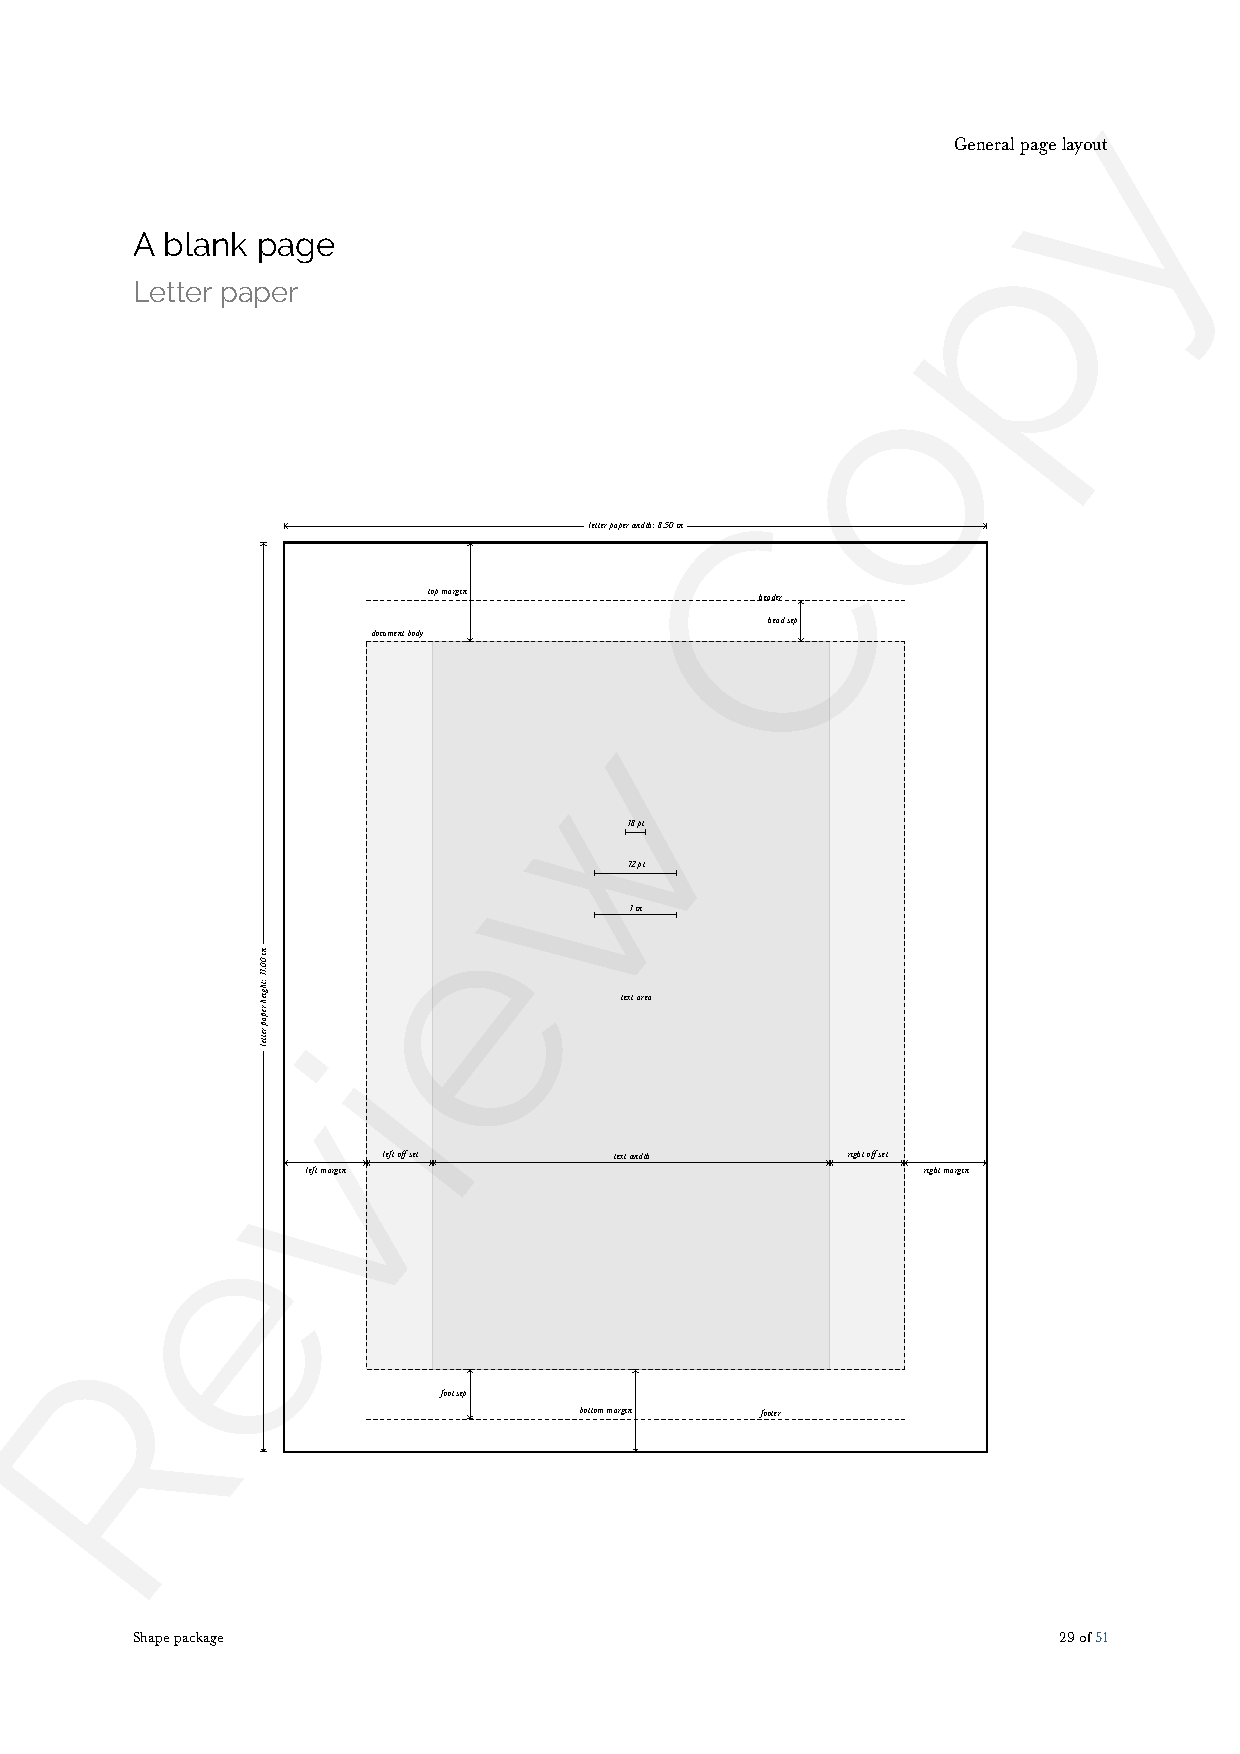
\includepdf{./FullPages/Layout1.pdf}
    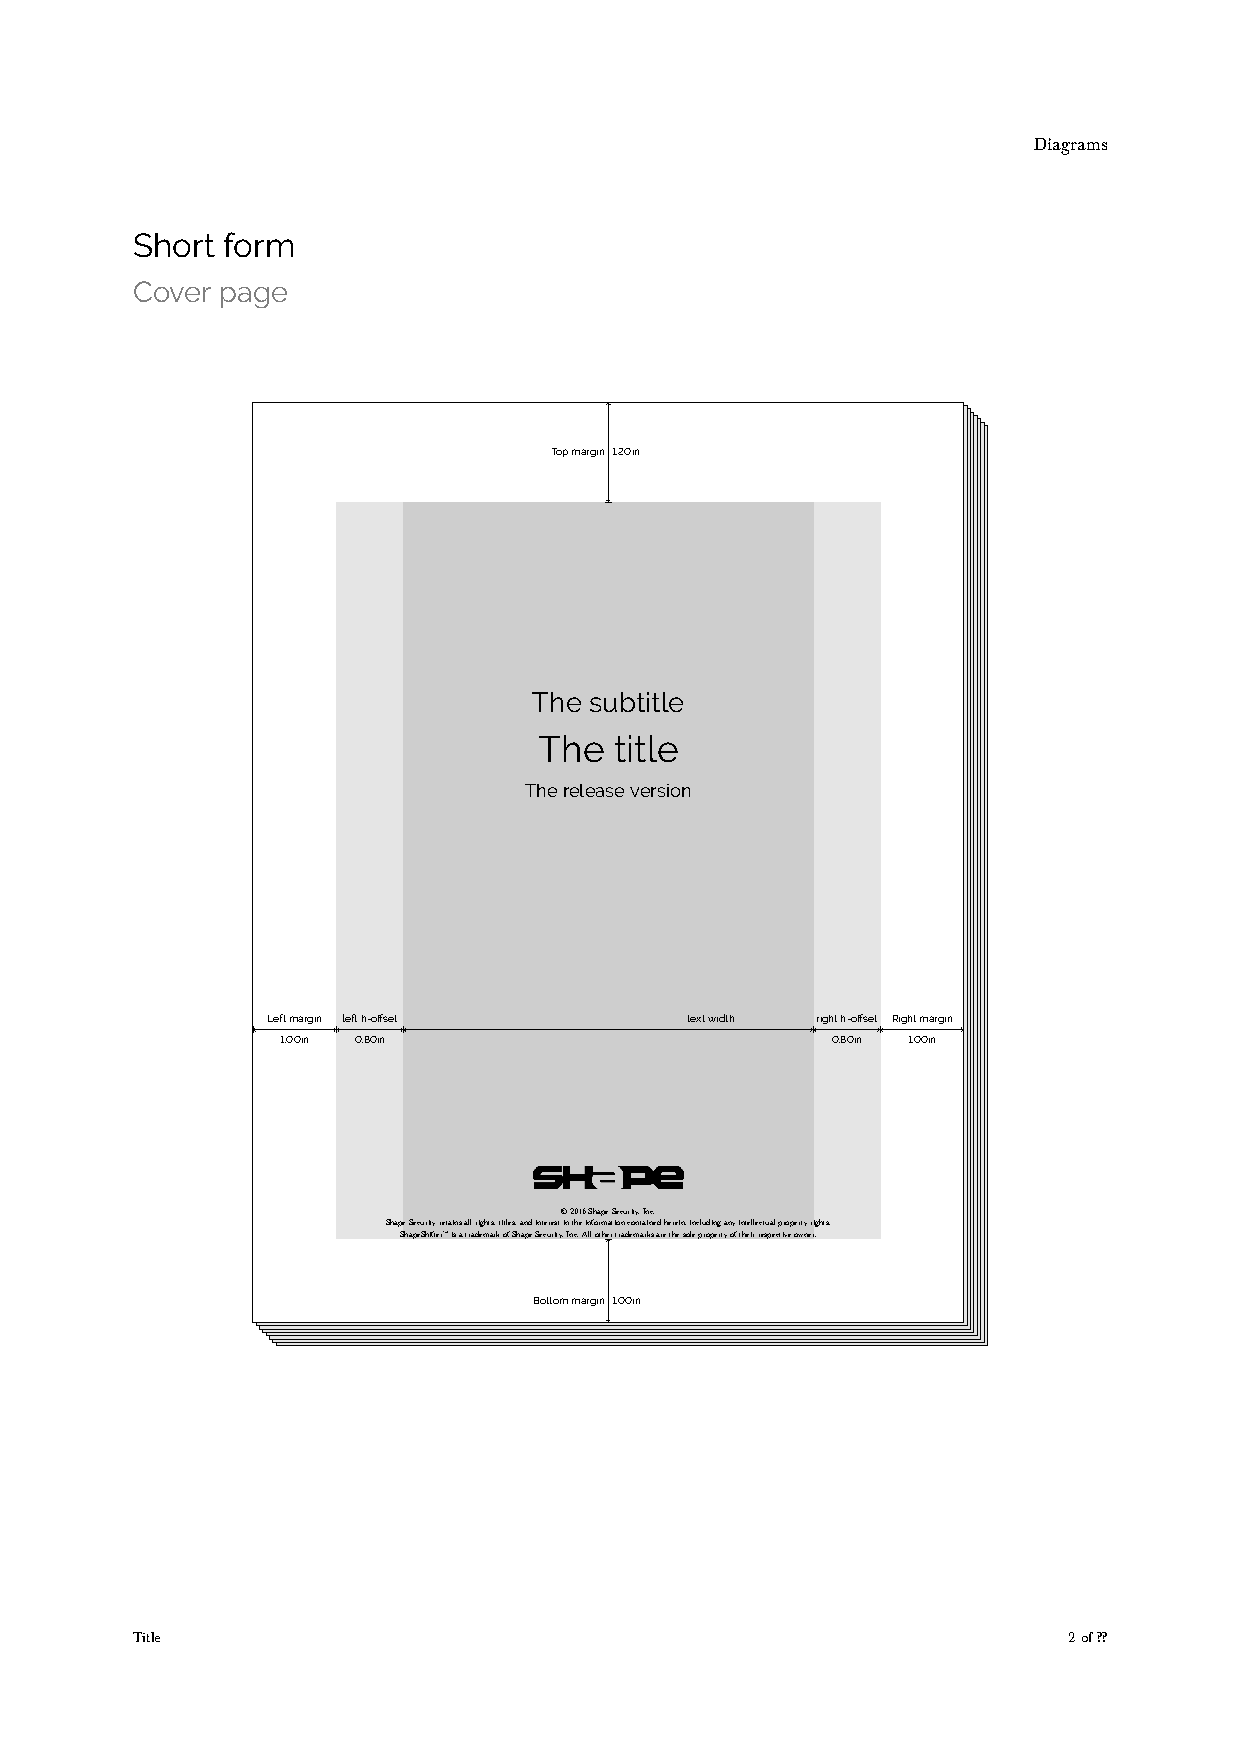
\includepdf{./FullPages/Layout2.pdf}
    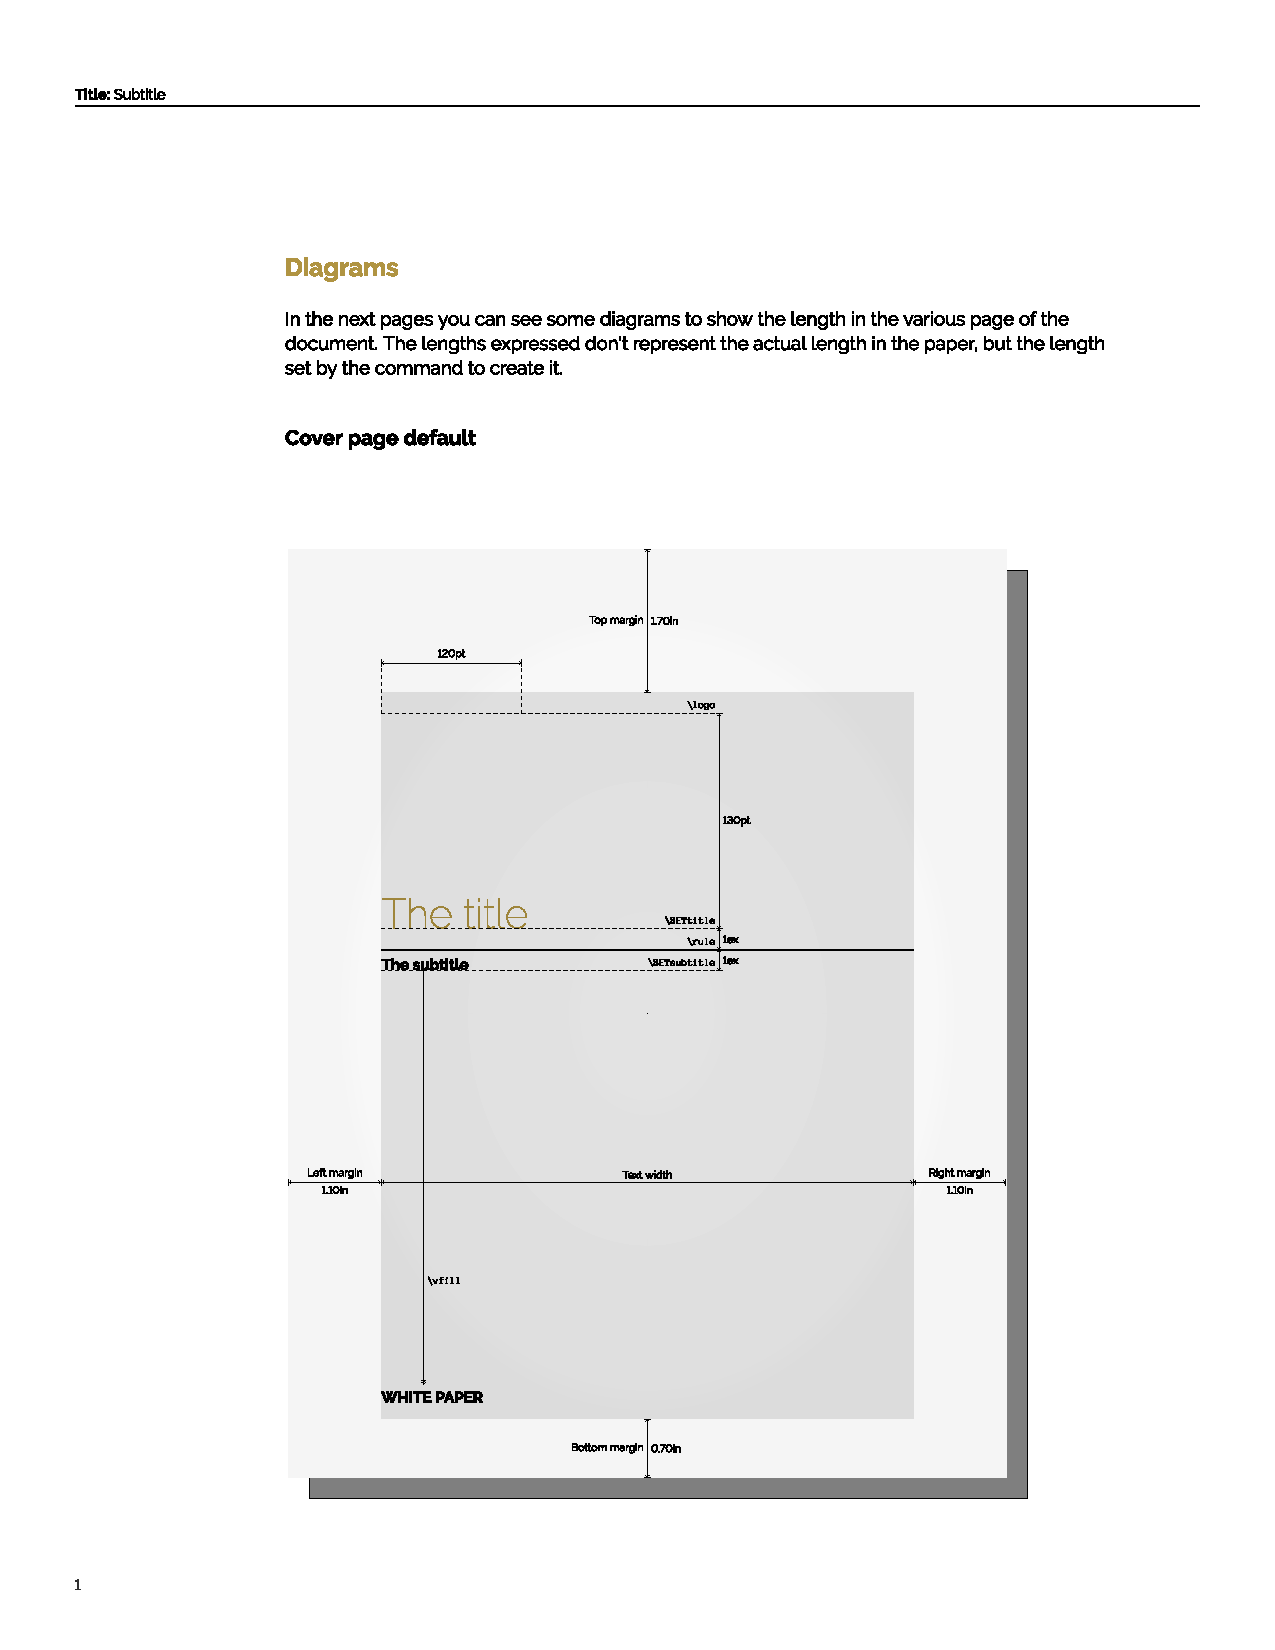
\includepdf{./FullPages/Layout3.pdf}
    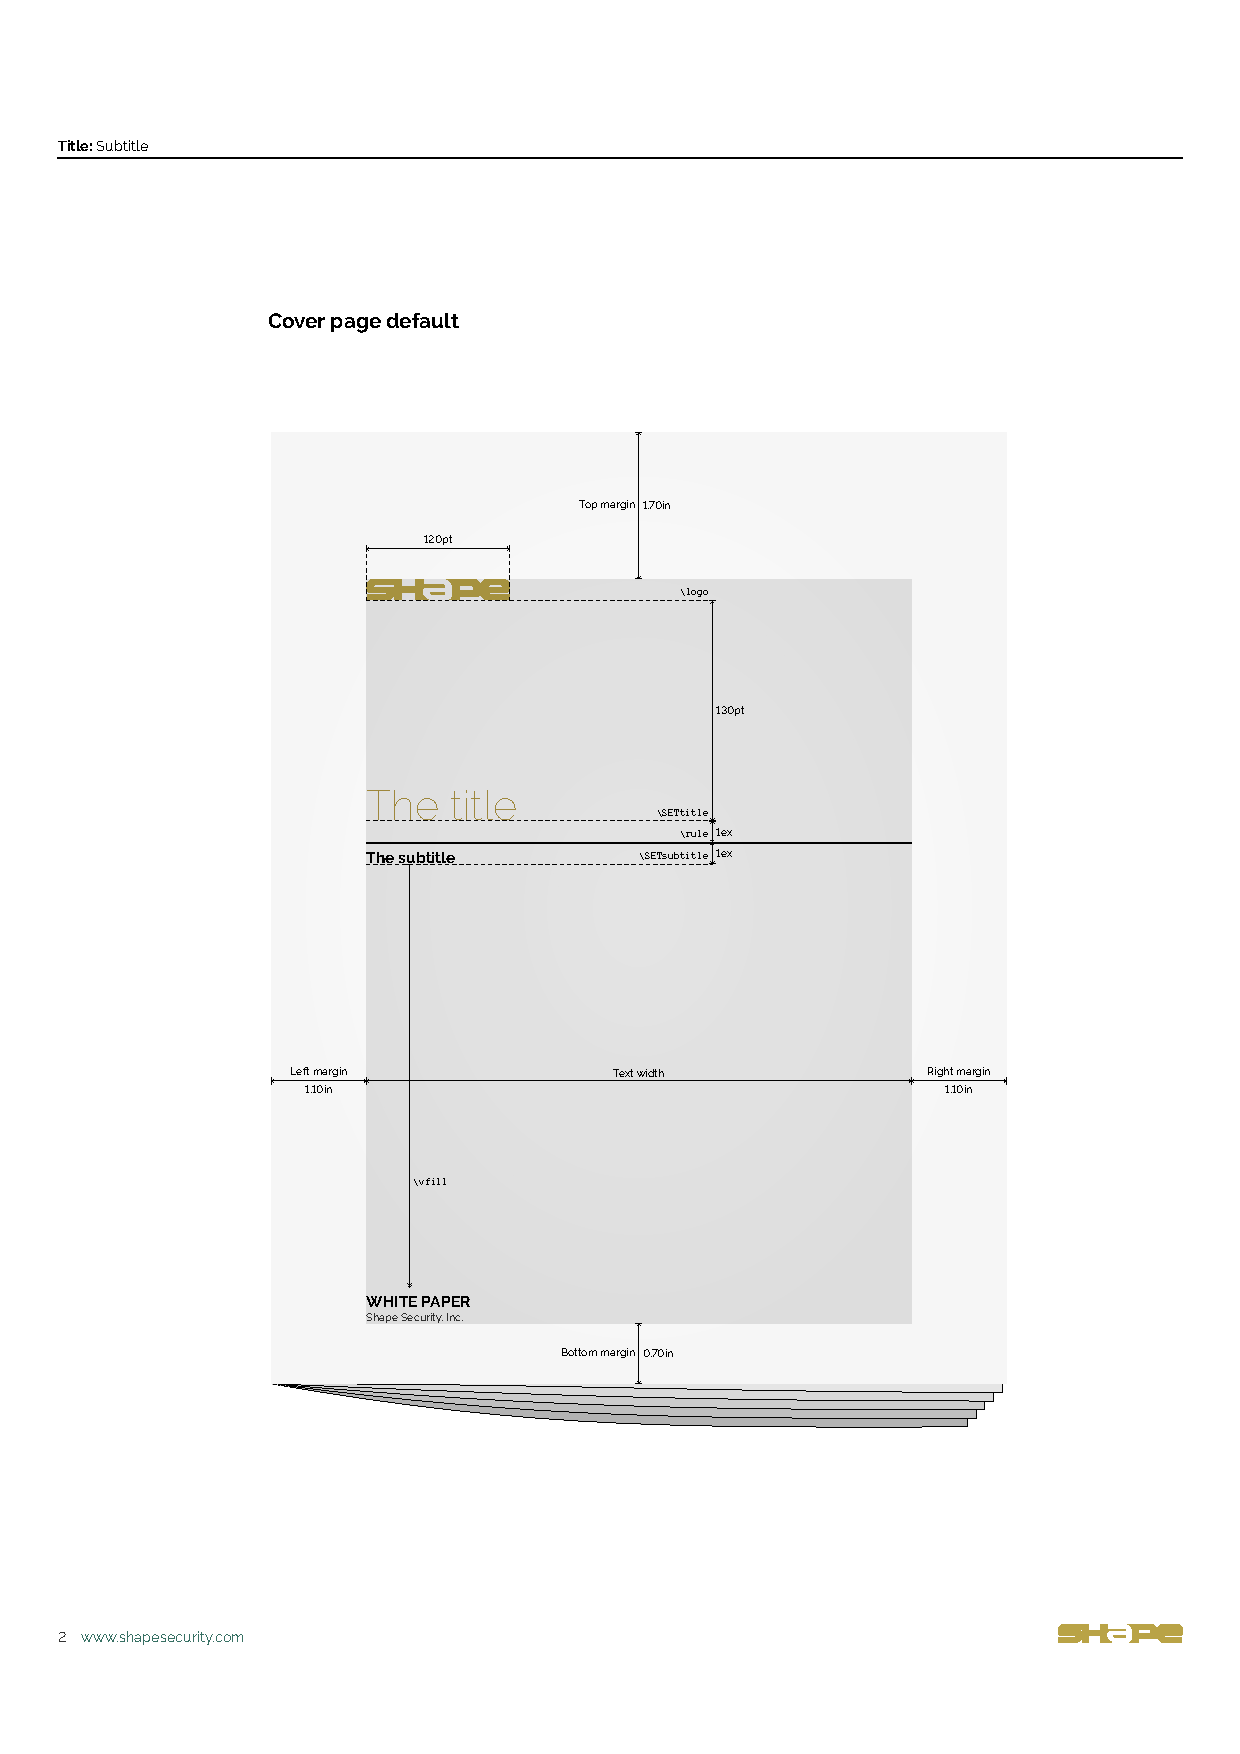
\includepdf{./FullPages/Layout4.pdf}

%%%%%%%%%%%%%%%%%%%%%%%%%%%%%%%%%%%%%%%%%%%%%%%%%%%%%%%%%%%%%%%%%%%%%
% Document conversions
%%%%%%%%%%%%%%%%%%%%%%%%%%%%%%%%%%%%%%%%%%%%%%%%%%%%%%%%%%%%%%%%%%%%%
    \titlefleuron{Document conversions}{\adfflowerleft}

    %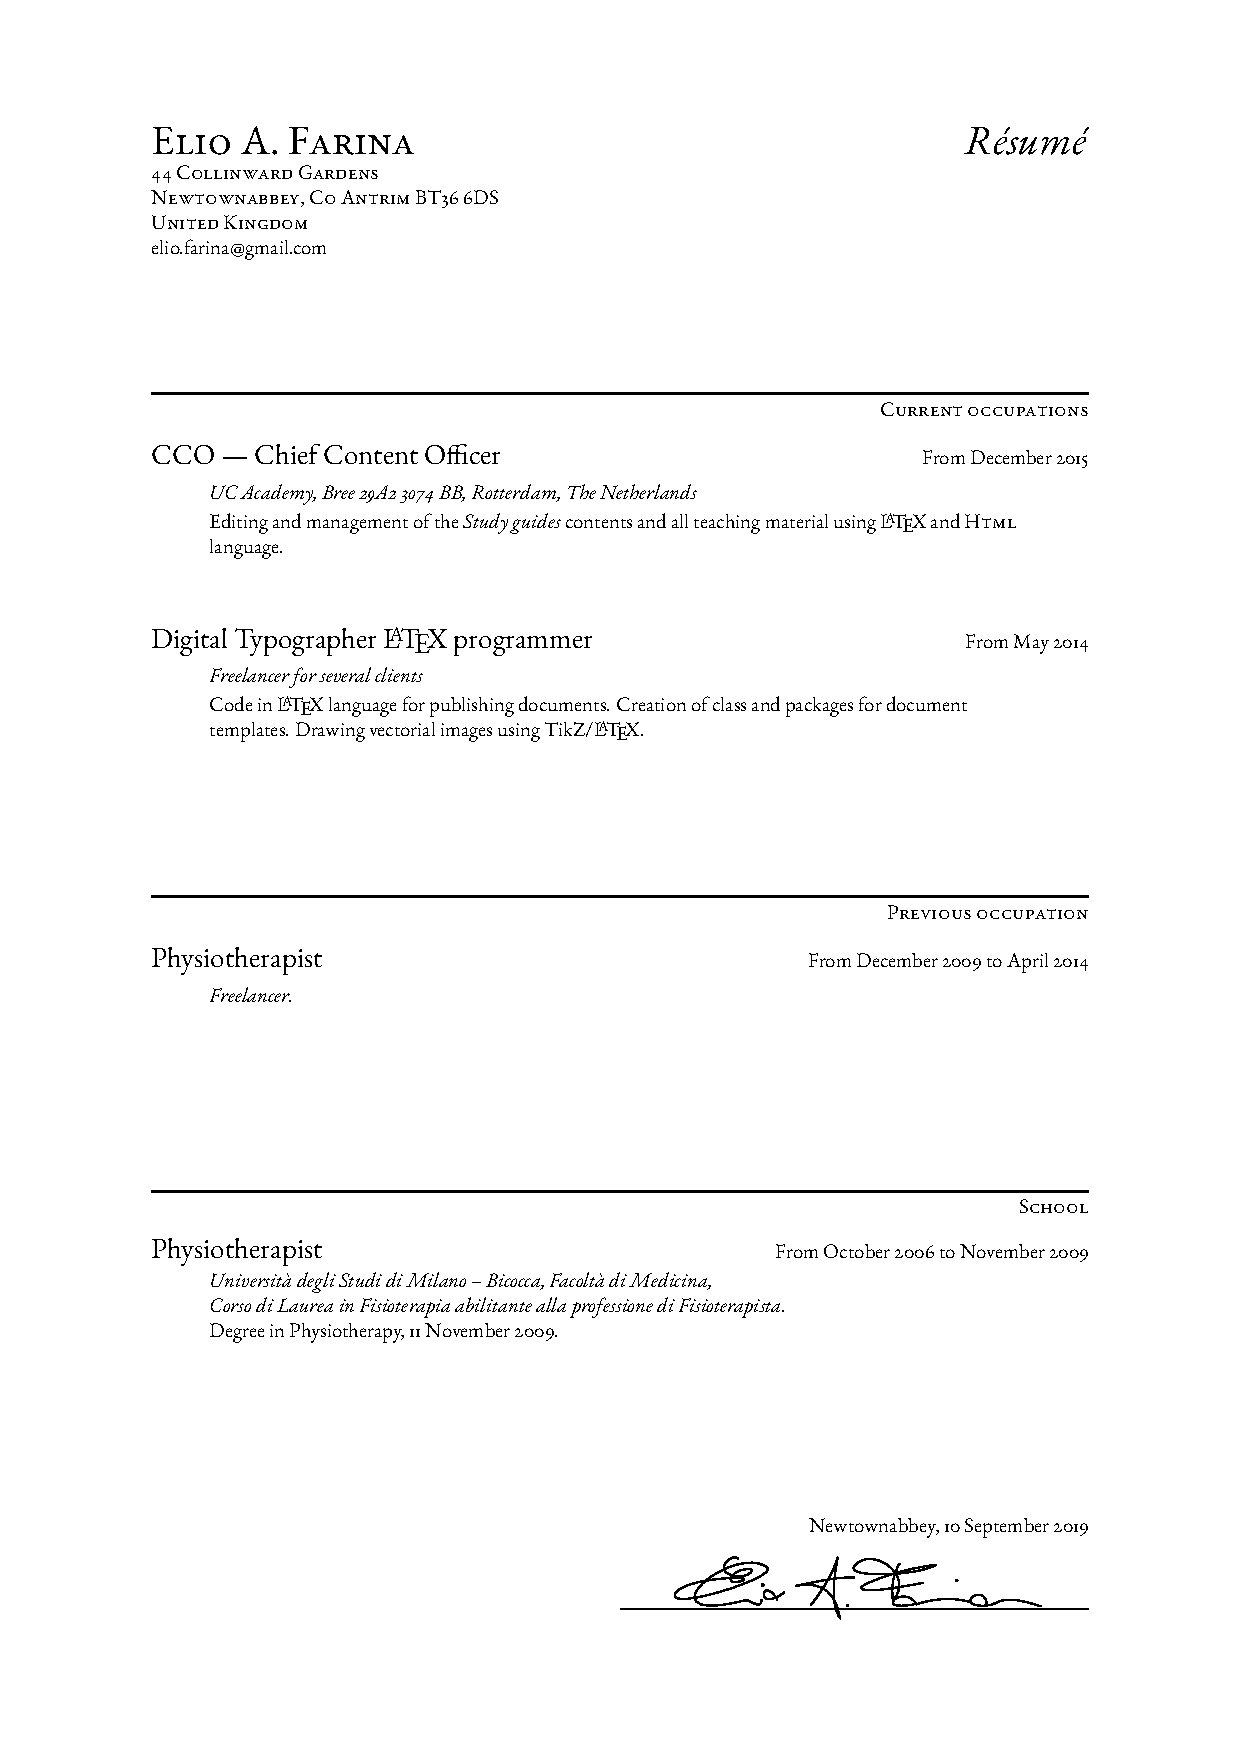
\includepdf{./FullPages/ResumeElioAFarinaEng.pdf}
    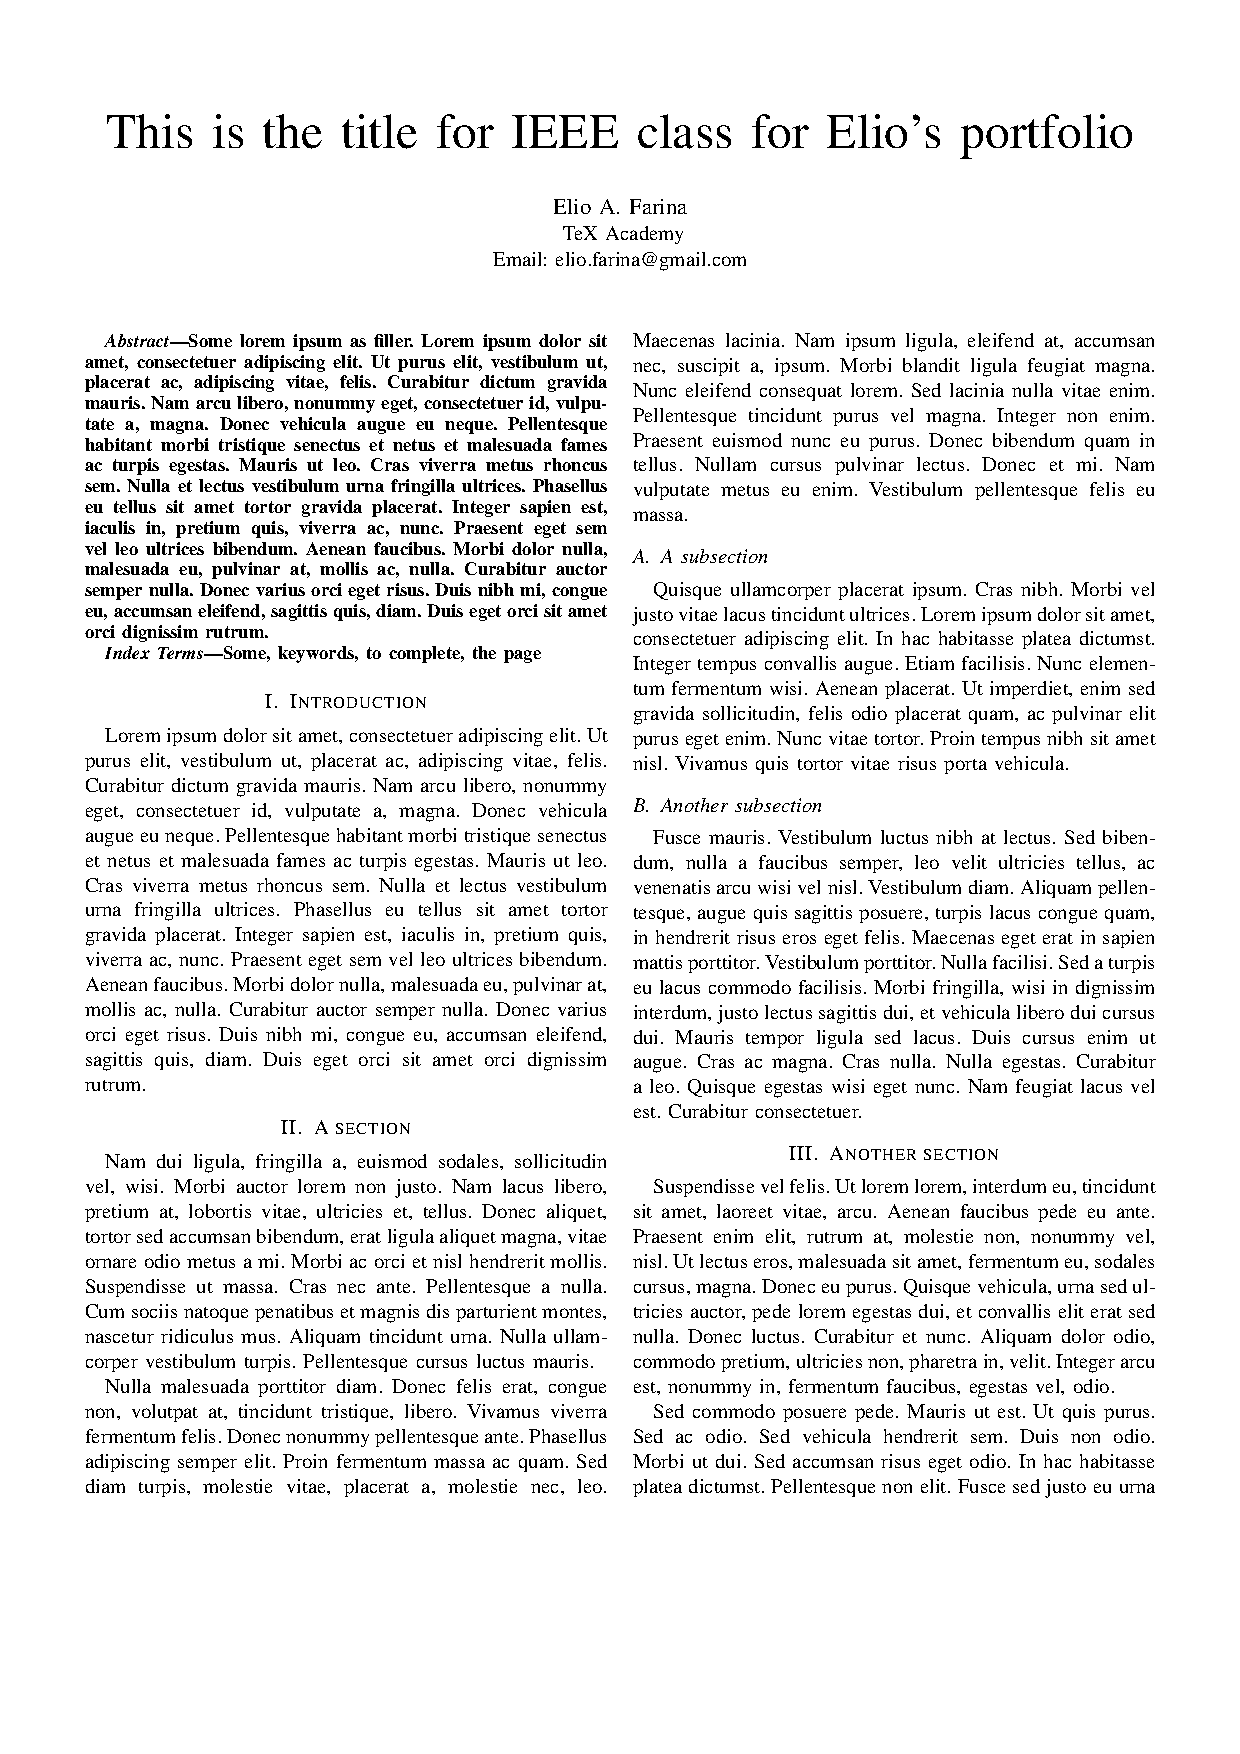
\includepdf{./FullPages/IEEE.pdf}
    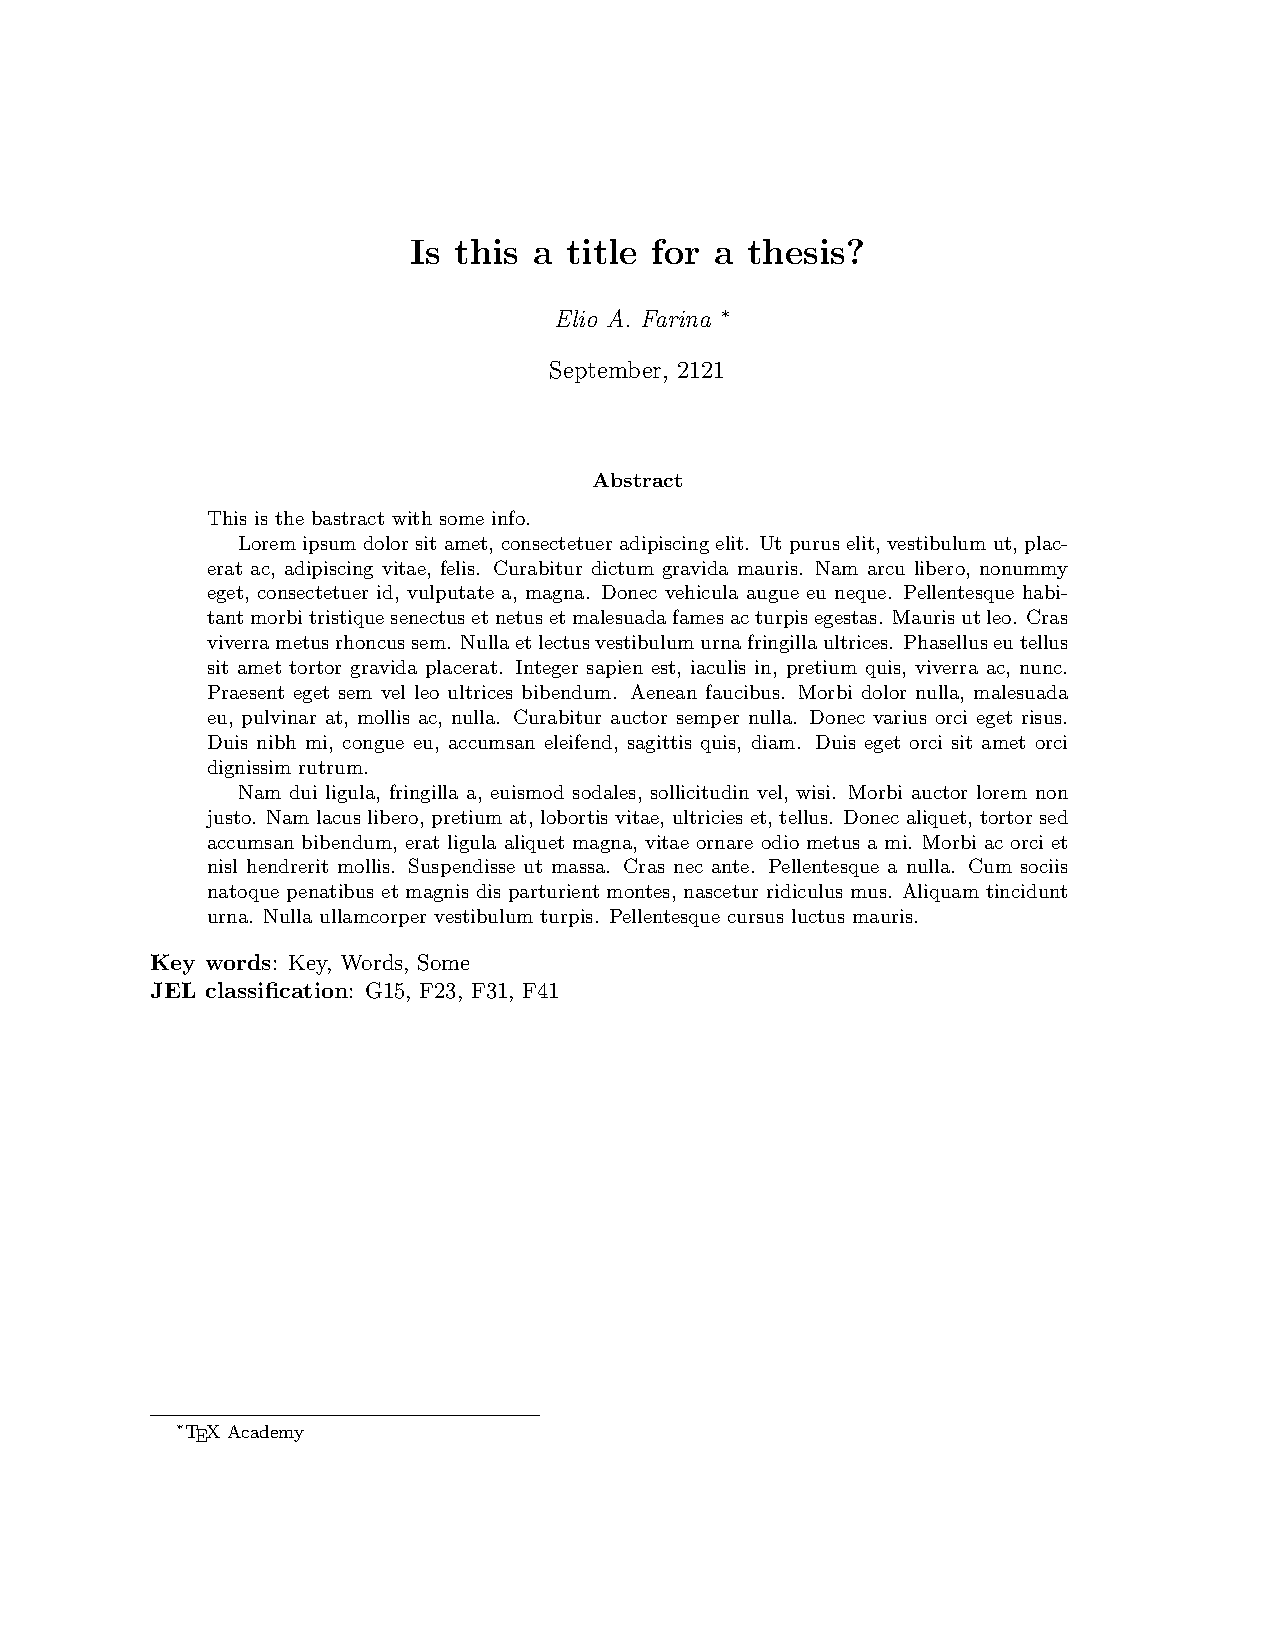
\includepdf{./FullPages/Thesis.pdf}
    
\includepdf{./FullPages/CoverMasterThesis.pdf}
    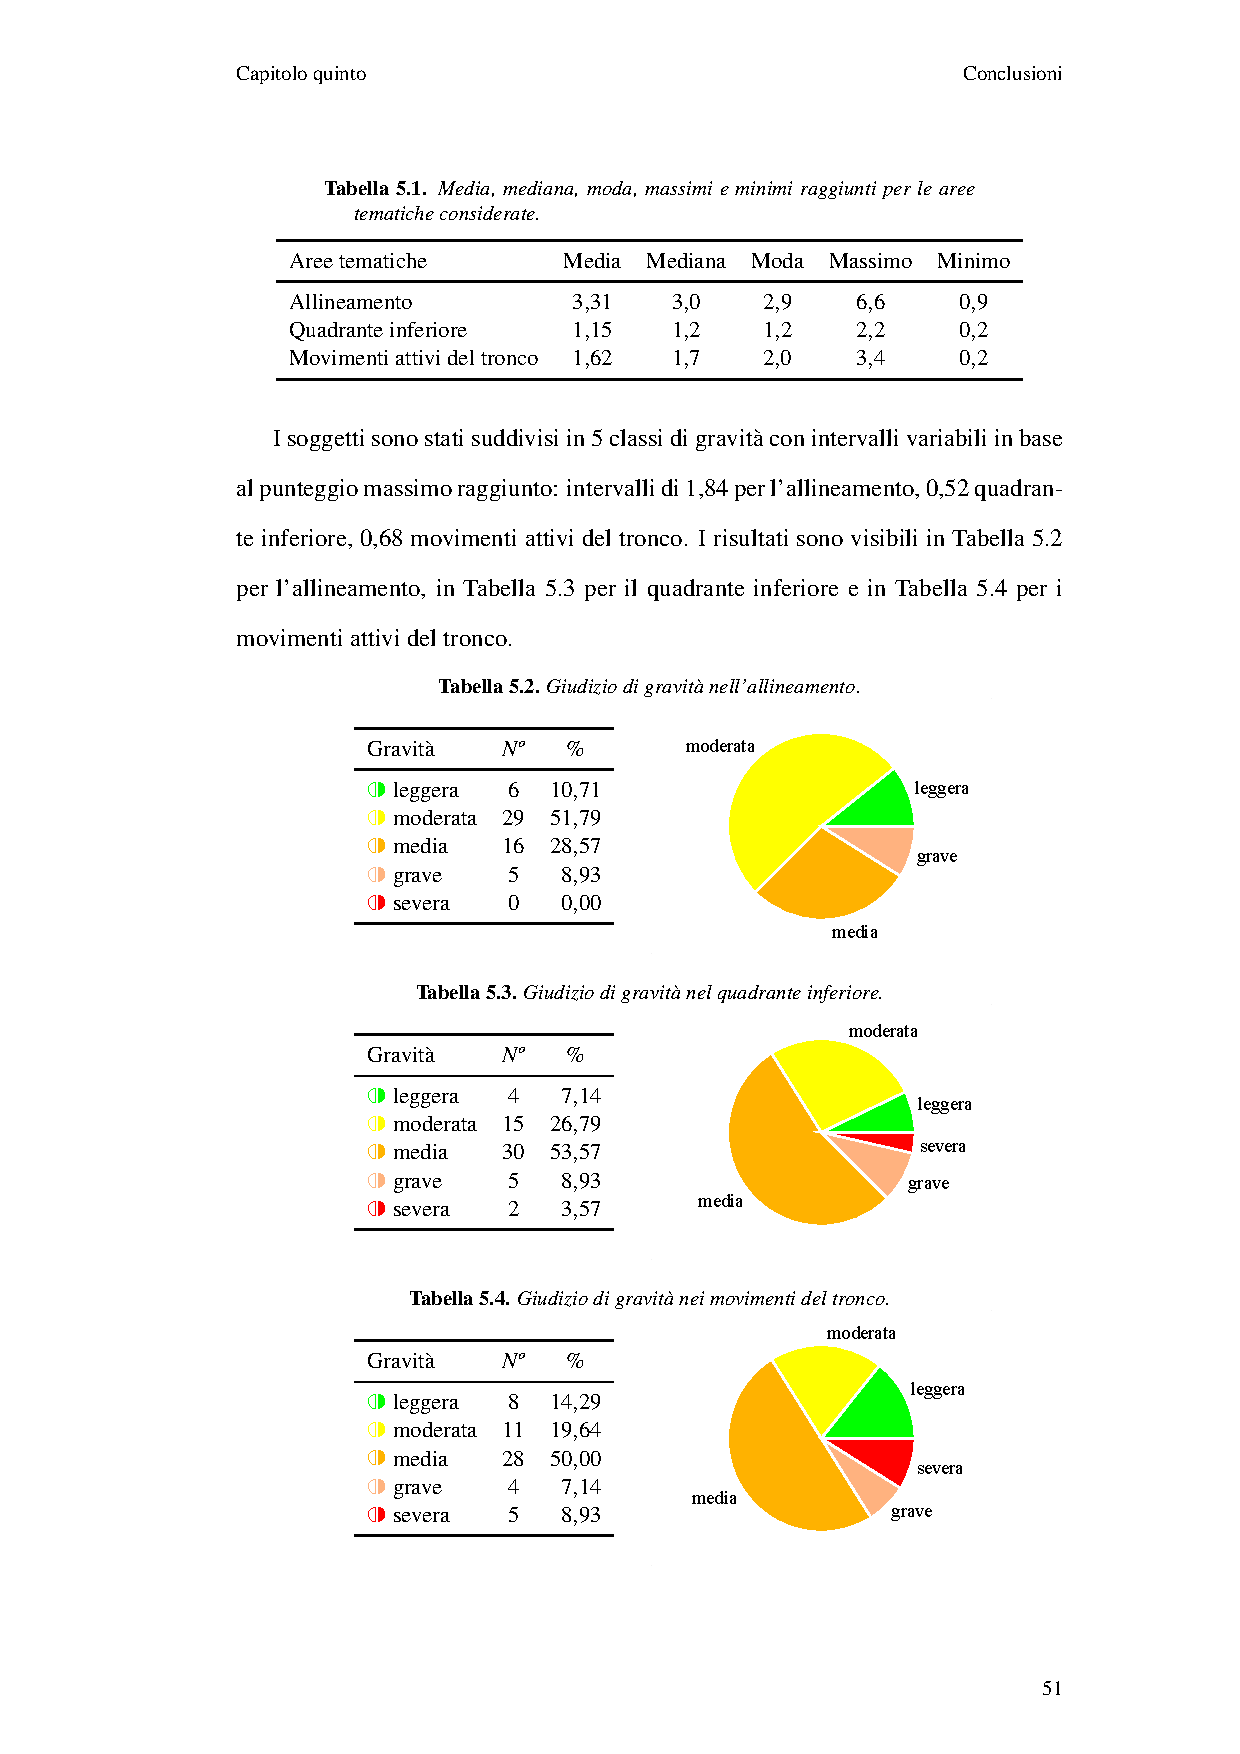
\includepdf{./FullPages/Thesis1.pdf}

%%%%%%%%%%%%%%%%%%%%%%%%%%%%%%%%%%%%%%%%%%%%%%%%%%%%%%%%%%%%%%%%%%%%%
% TikZ works
%%%%%%%%%%%%%%%%%%%%%%%%%%%%%%%%%%%%%%%%%%%%%%%%%%%%%%%%%%%%%%%%%%%%%
    \titlenofleuron{TikZ works}{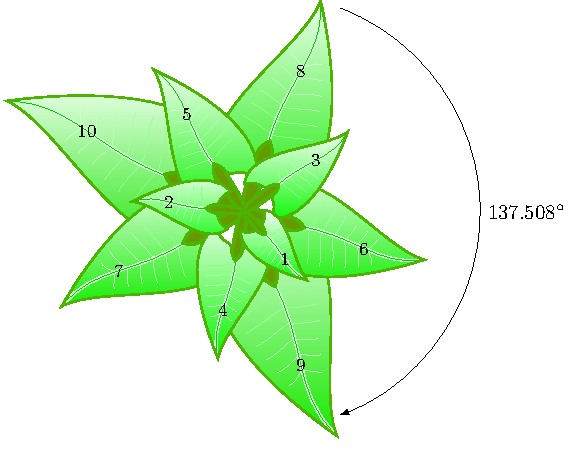
\includegraphics{./TikZimages/TikZ1.pdf}}

    \begin{minipage}{0.475\linewidth}\centering
            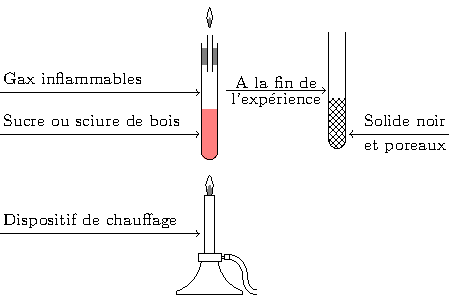
\includegraphics[width=\linewidth]{./TikZimages/TikZ2.pdf}
        \end{minipage}\hfill\begin{minipage}{0.475\linewidth}\centering
            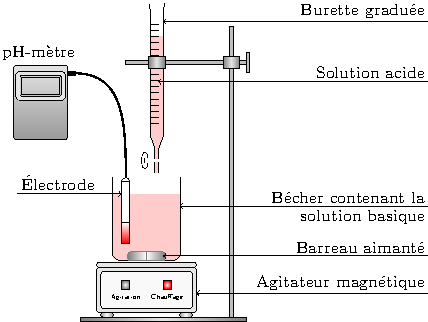
\includegraphics[width=\linewidth]{./TikZimages/TikZ3.pdf}\\
    \end{minipage}

    \vfill
    \begin{minipage}{0.475\linewidth}\centering
            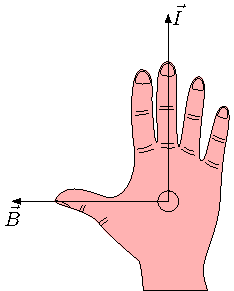
\includegraphics{./TikZimages/TikZ4.pdf}
        \end{minipage}\hfill\begin{minipage}{0.475\linewidth}\centering
            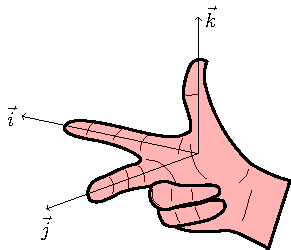
\includegraphics{./TikZimages/TikZ6.pdf}\\
    \end{minipage}

    \vfill
    \begin{minipage}{\linewidth}\centering
    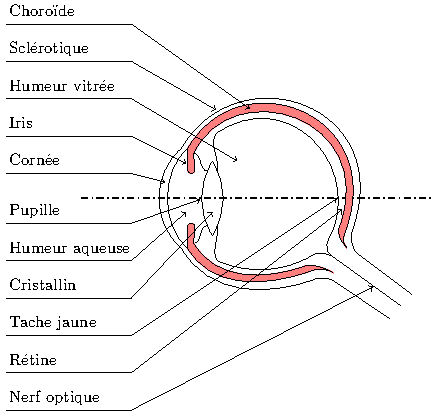
\includegraphics{./TikZimages/TikZ5.pdf}\\
    \end{minipage}

    \clearpage
    \begin{center}
        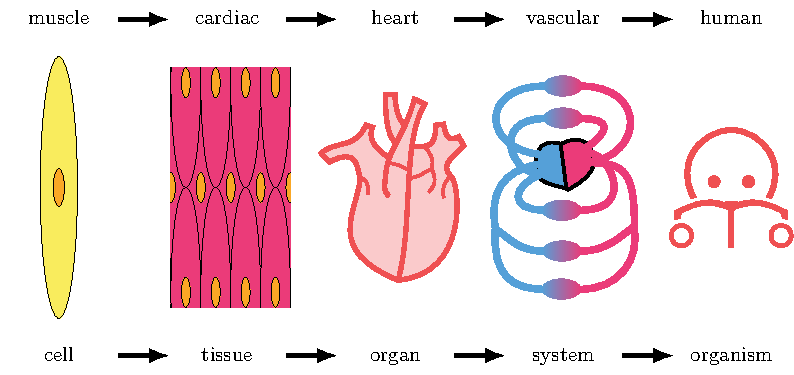
\includegraphics[width=0.85\linewidth]{./TikZimages/TikZ10.pdf}\\
        \vfill
        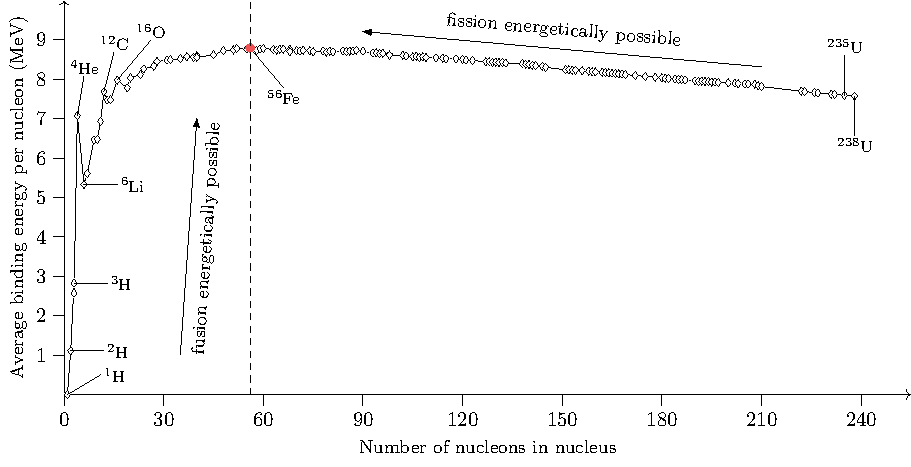
\includegraphics[width=0.85\linewidth]{./TikZimages/TikZ12.pdf}\\
        \vfill
        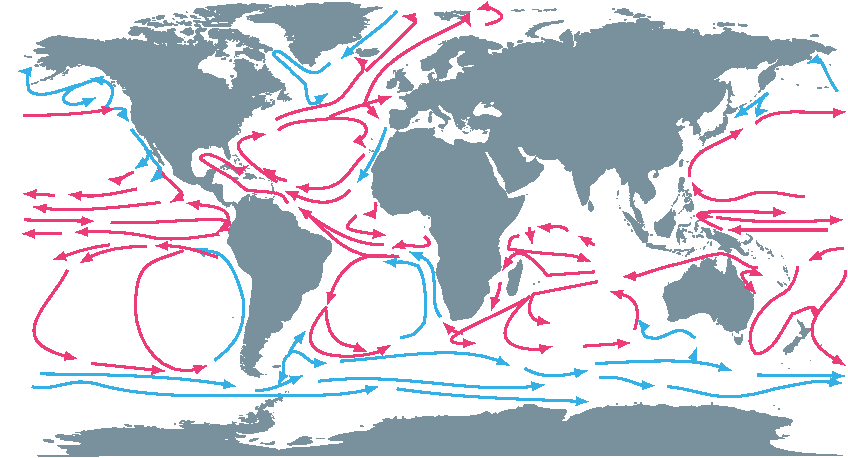
\includegraphics[width=0.85\linewidth]{./TikZimages/TikZ11.pdf}
    \end{center}

    \clearpage
    \begin{center}
        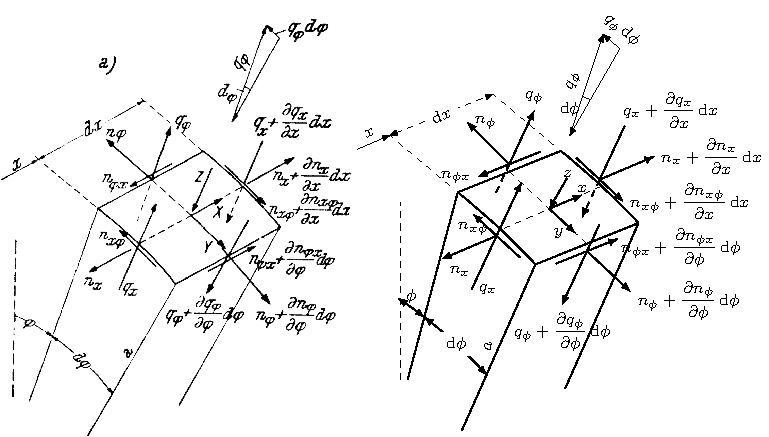
\includegraphics[width=0.8\linewidth]{./TikZimages/TikZ7.pdf}\\
        \vfill
        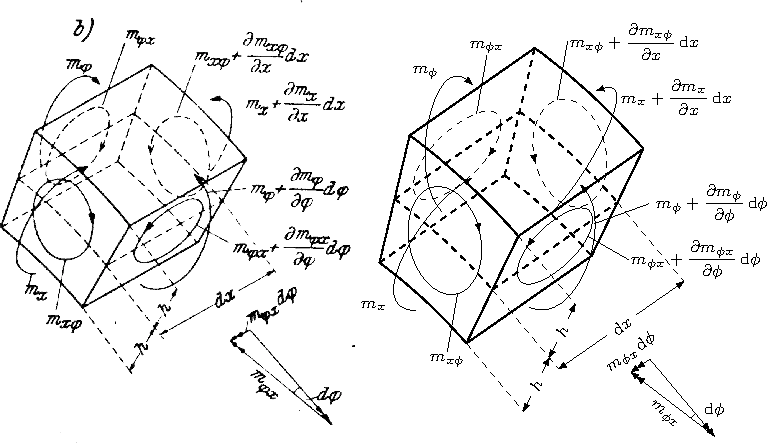
\includegraphics[width=0.8\linewidth]{./TikZimages/TikZ8.pdf}\\
        \vfill
        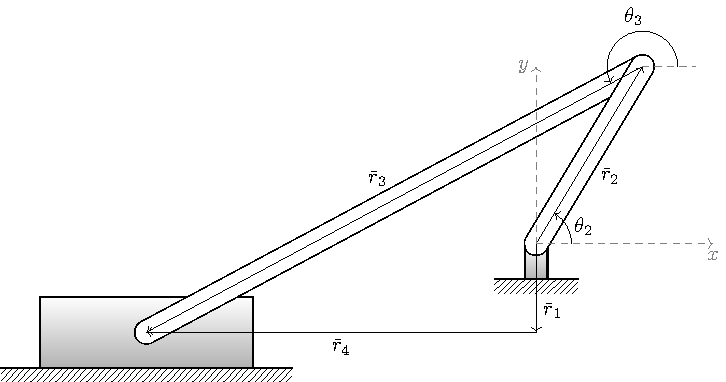
\includegraphics[width=0.8\linewidth]{./TikZimages/TikZ9.pdf}
    \end{center}

    \clearpage
    \begin{center}
    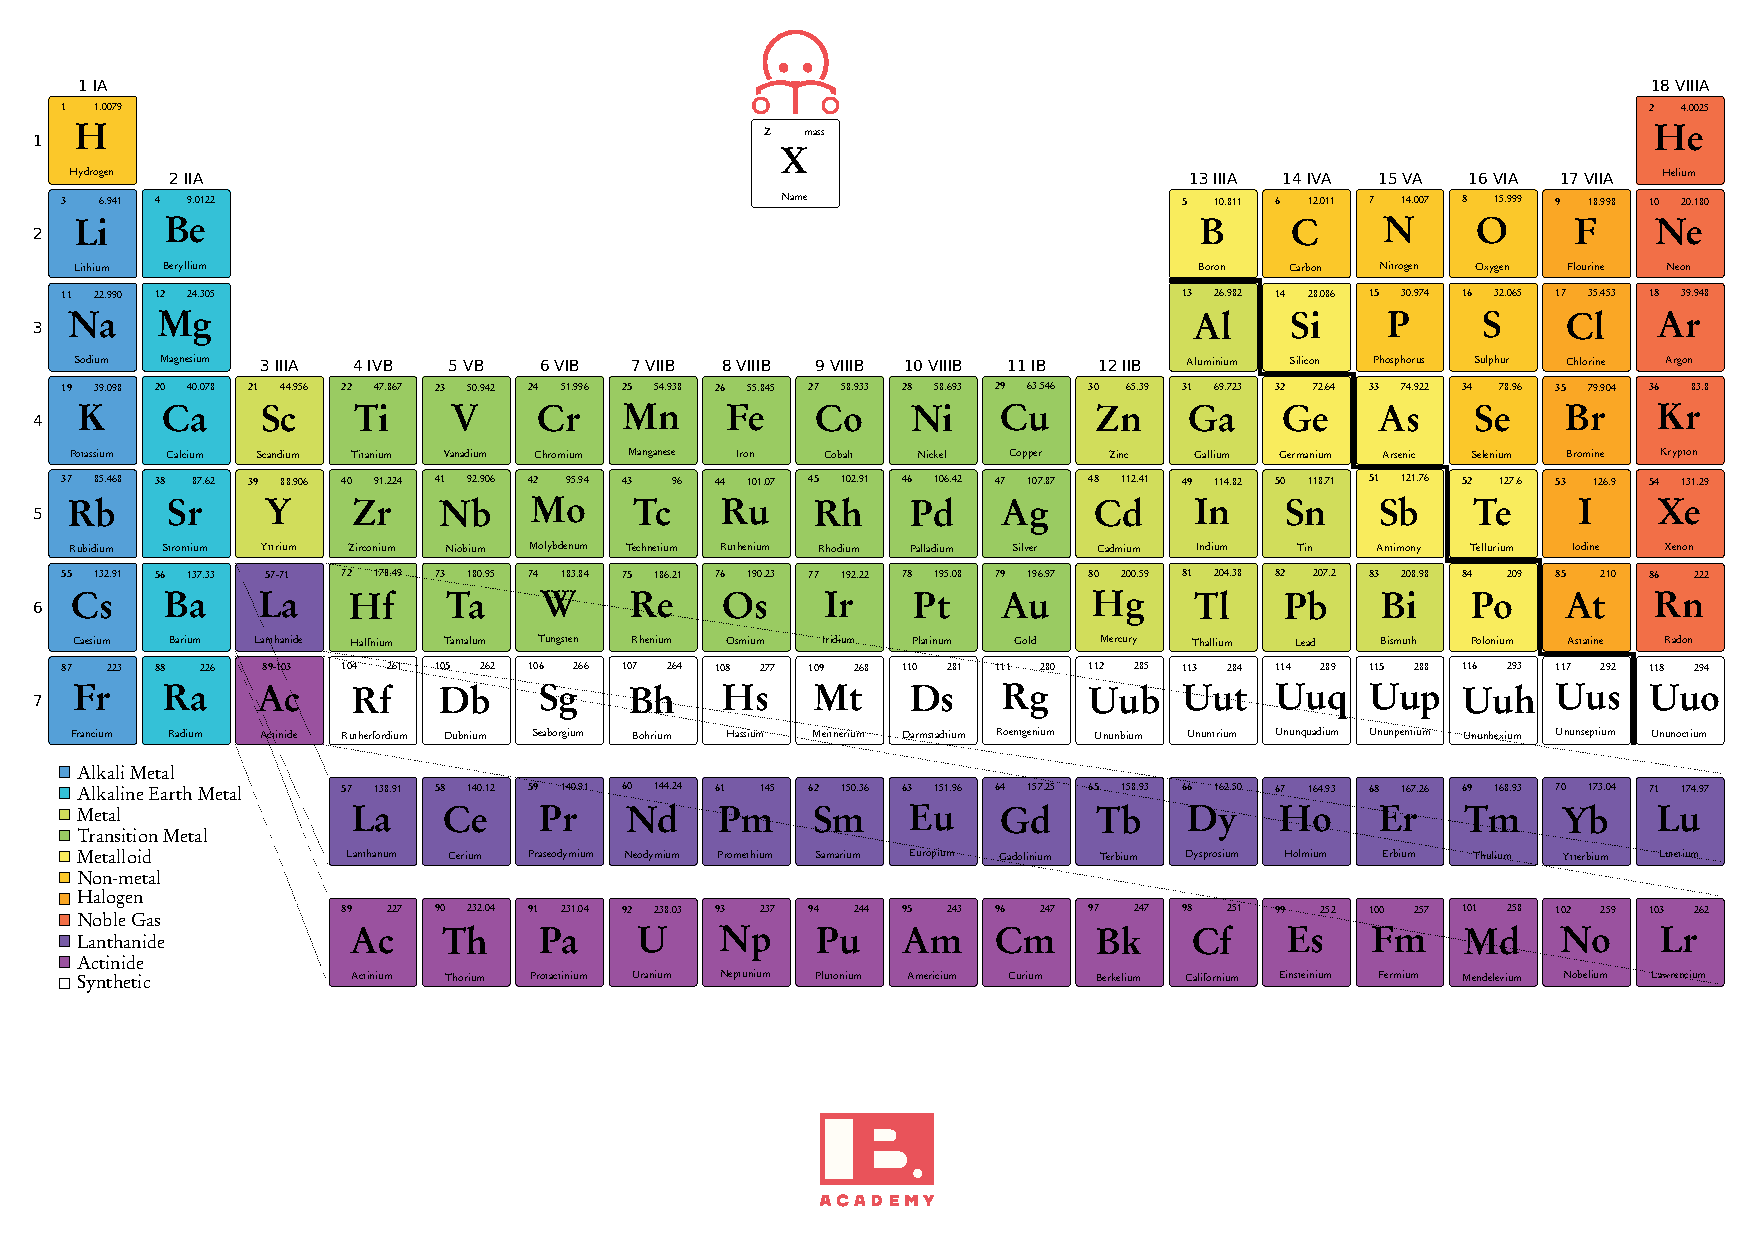
\includegraphics[height=\linewidth,angle=90]{./FullPages/TPE.pdf}
    \end{center}

%%%%%%%%%%%%%%%%%%%%%%%%%%%%%%%%%%%%%%%%%%%%%%%%%%%%%%%%%%%%%%%%%%%%%
% Page samples
%%%%%%%%%%%%%%%%%%%%%%%%%%%%%%%%%%%%%%%%%%%%%%%%%%%%%%%%%%%%%%%%%%%%%
    \titlefleuron{Page samples}{\adfdownhalfleafleft}

    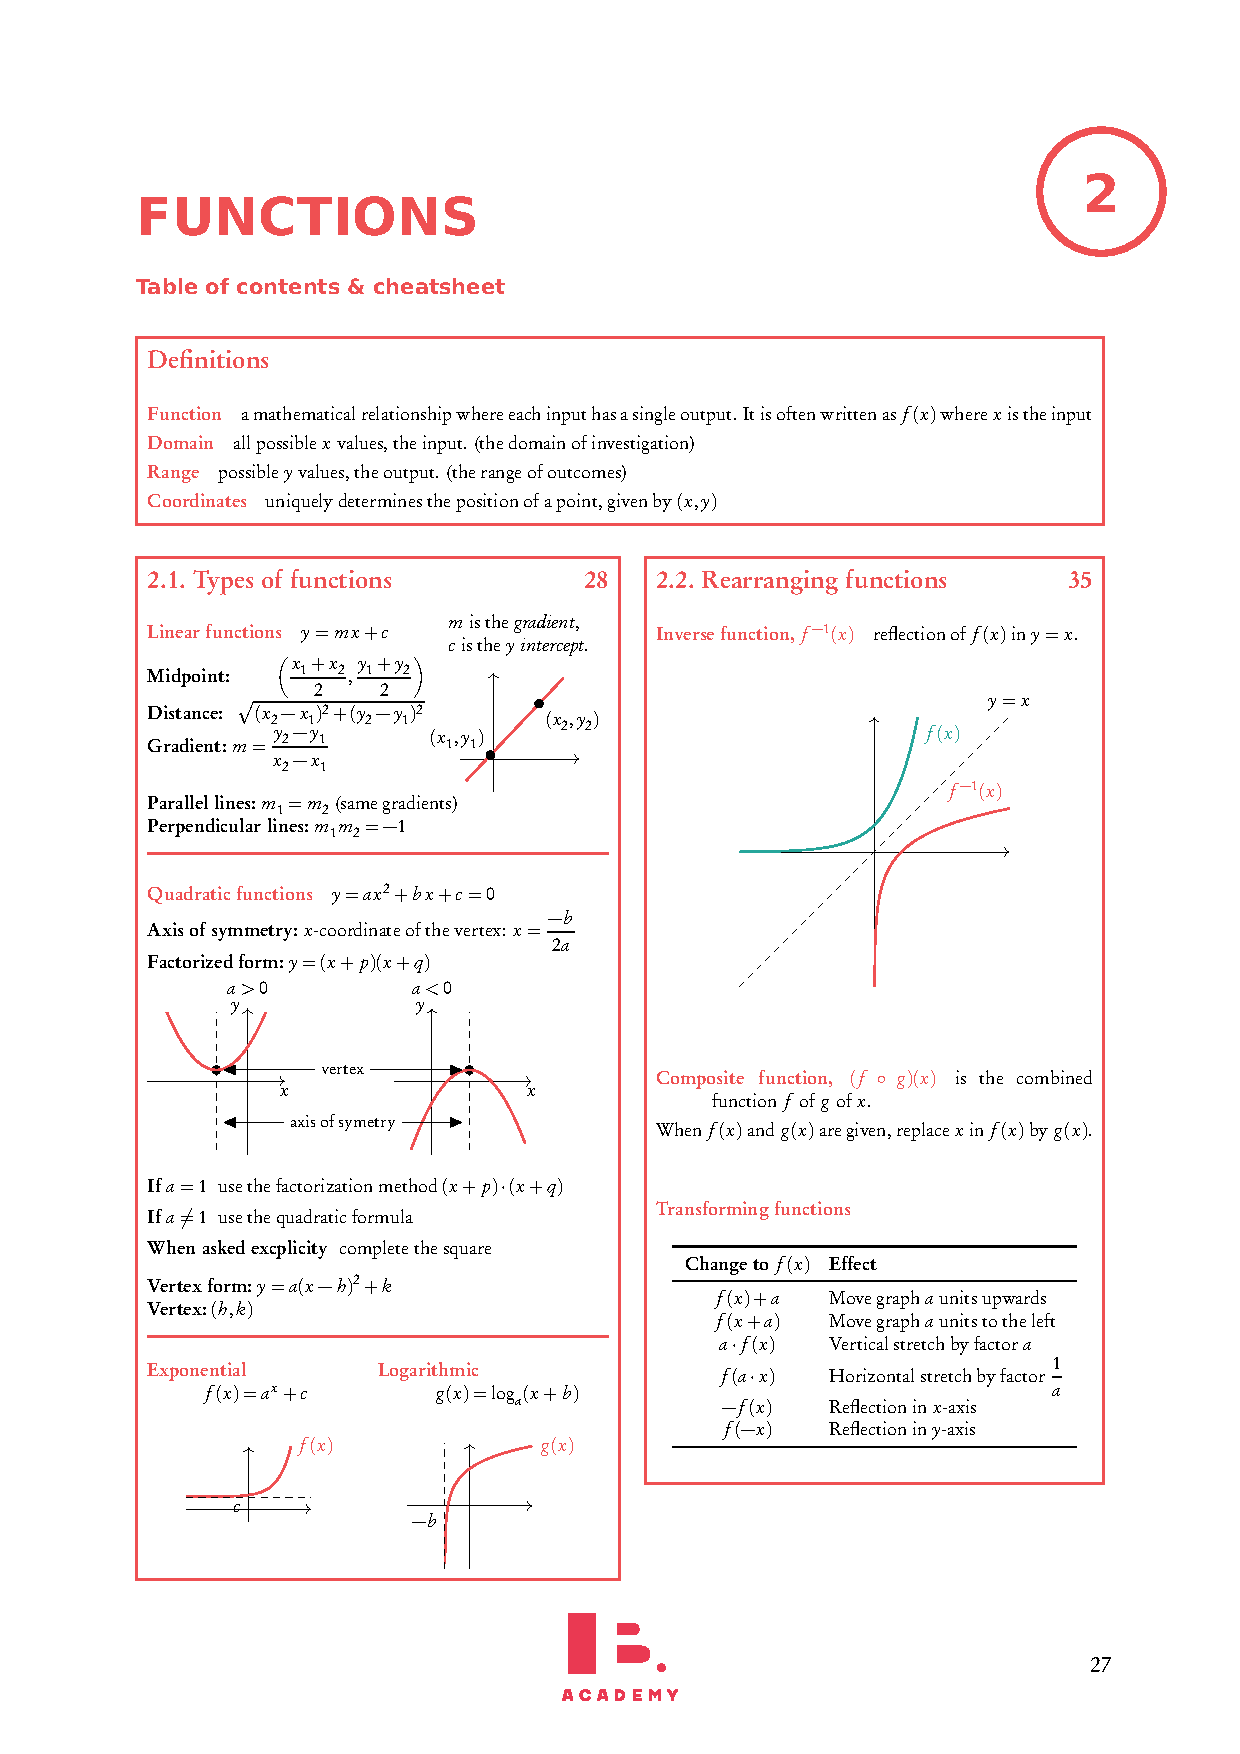
\includepdf{./FullPages/IBpage1.pdf}
    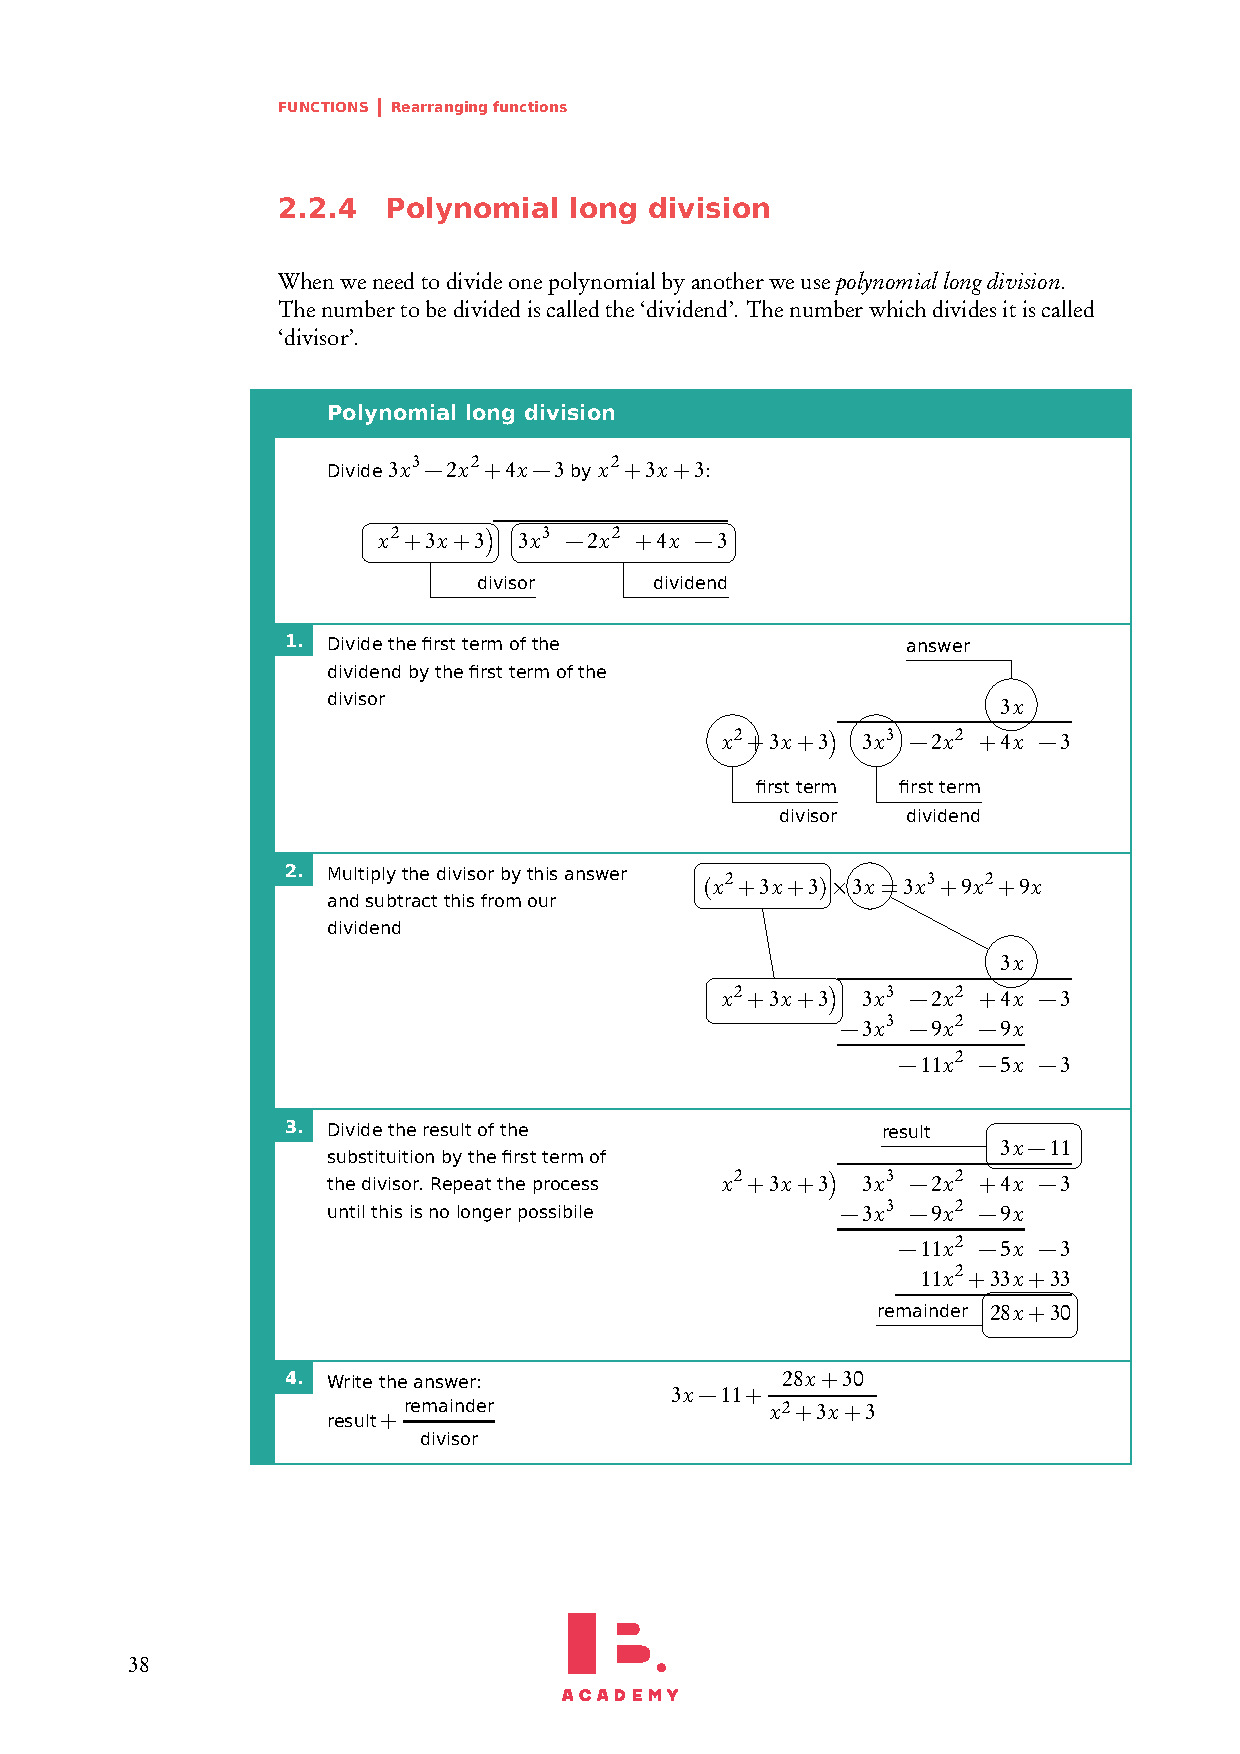
\includepdf{./FullPages/IBpage2.pdf}
    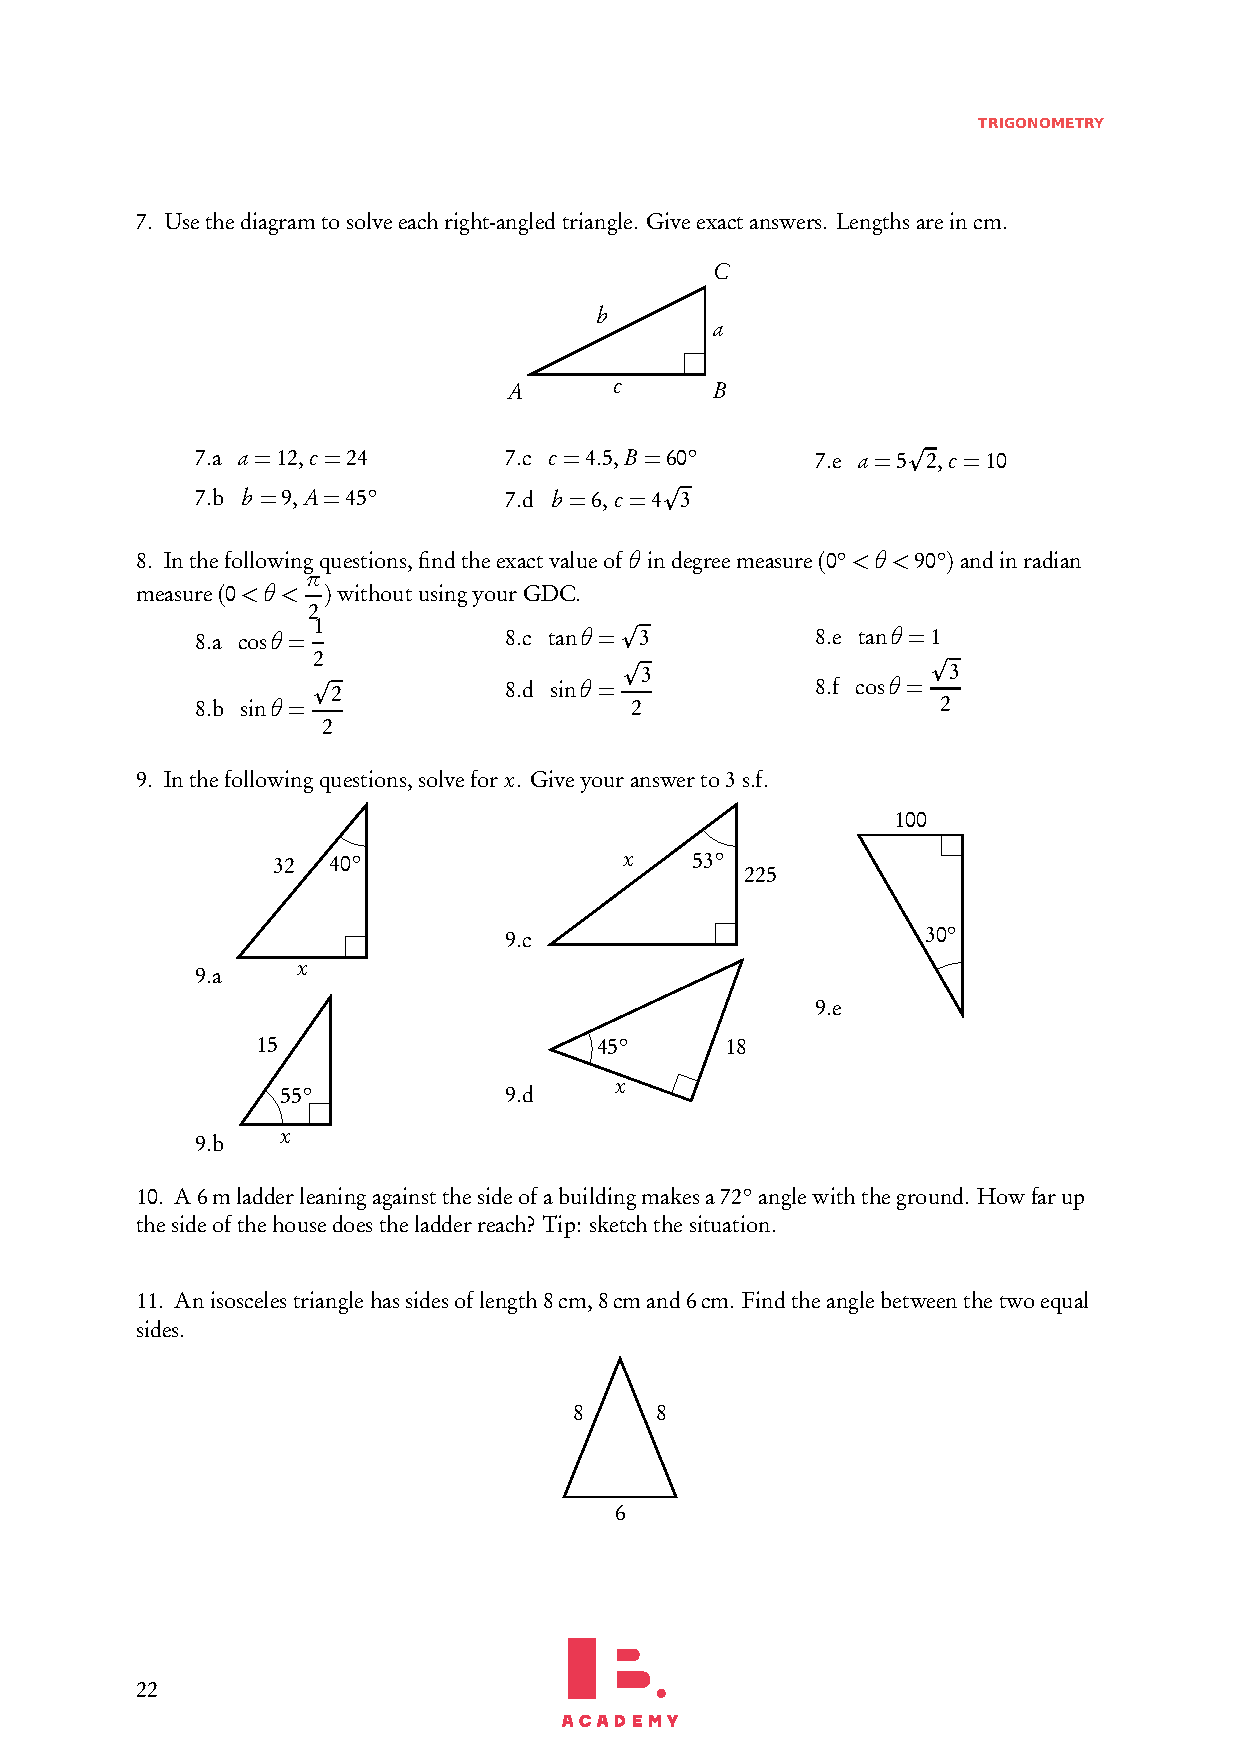
\includepdf{./FullPages/IBpage3.pdf}
    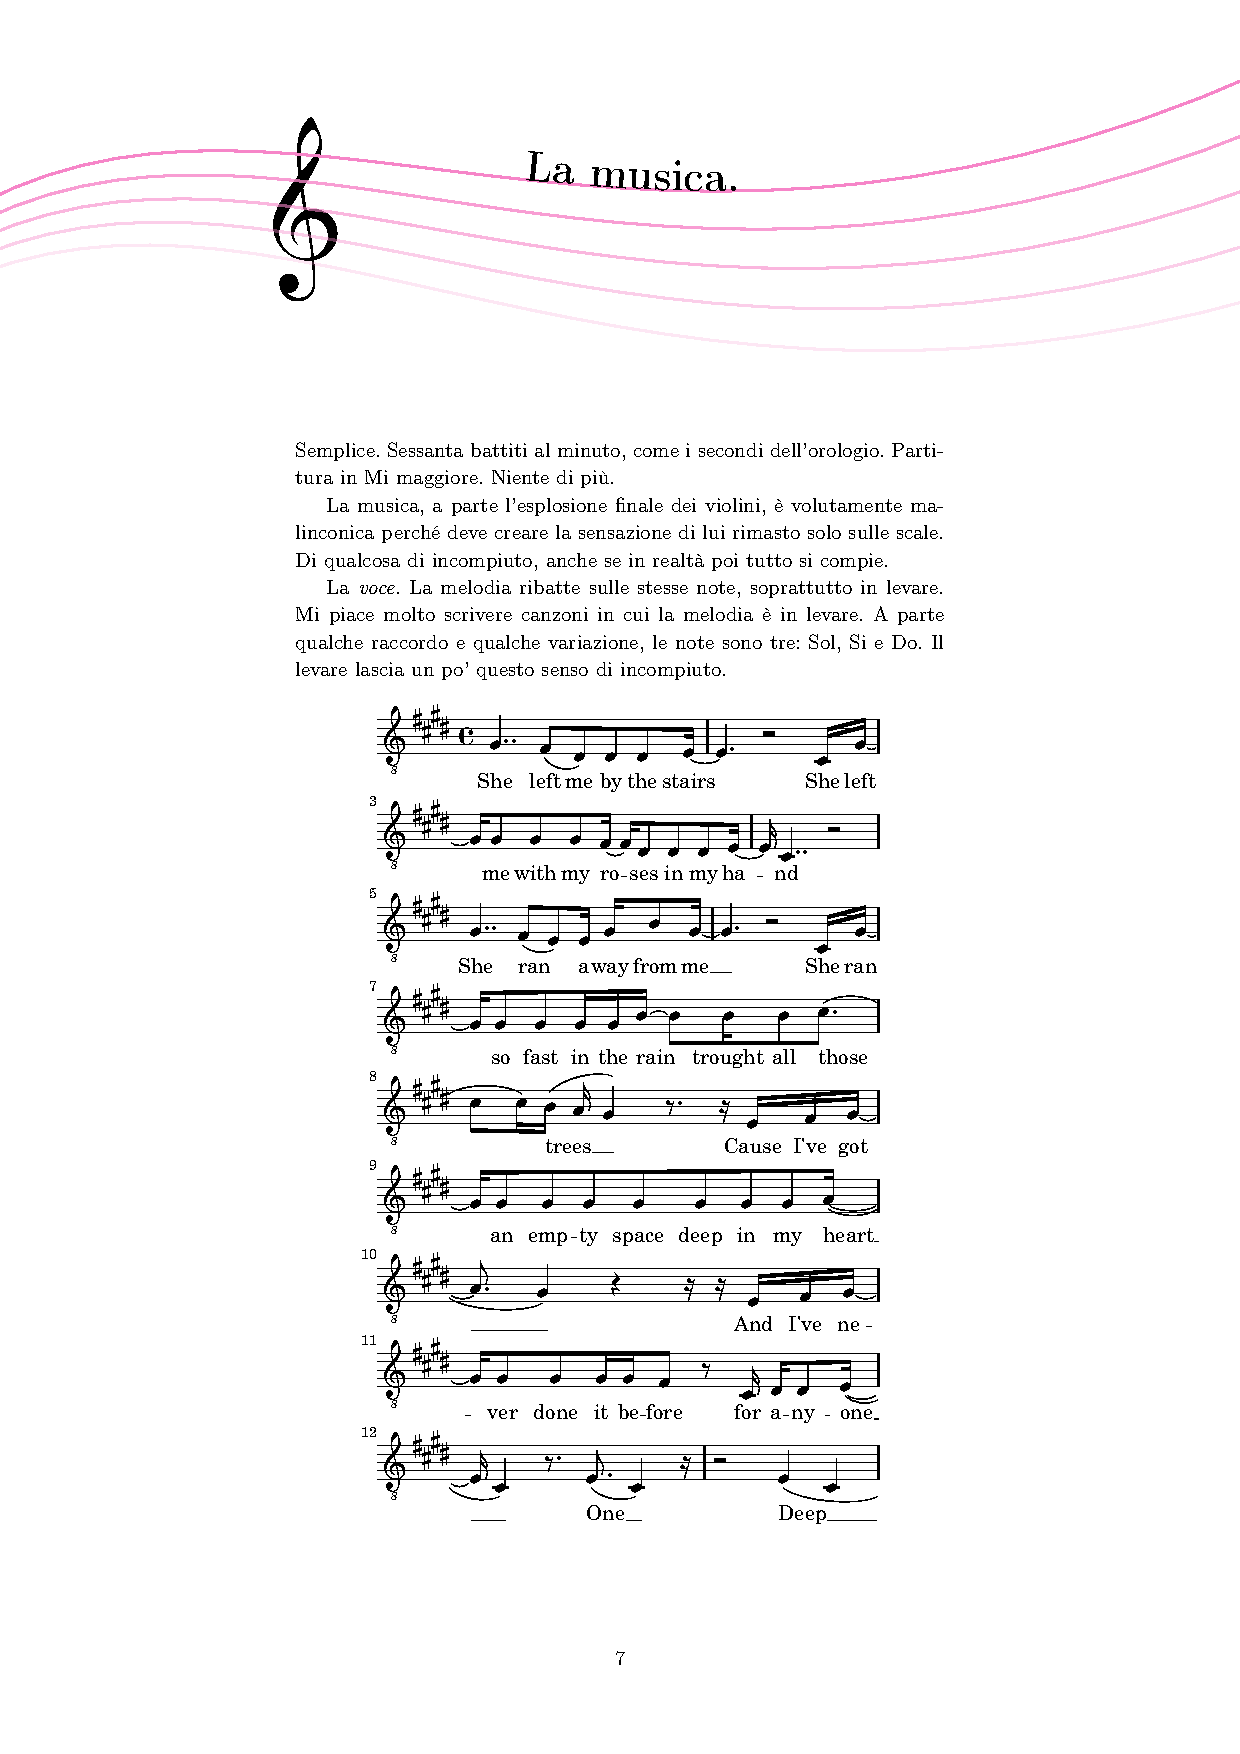
\includepdf{./FullPages/Music1.pdf}
    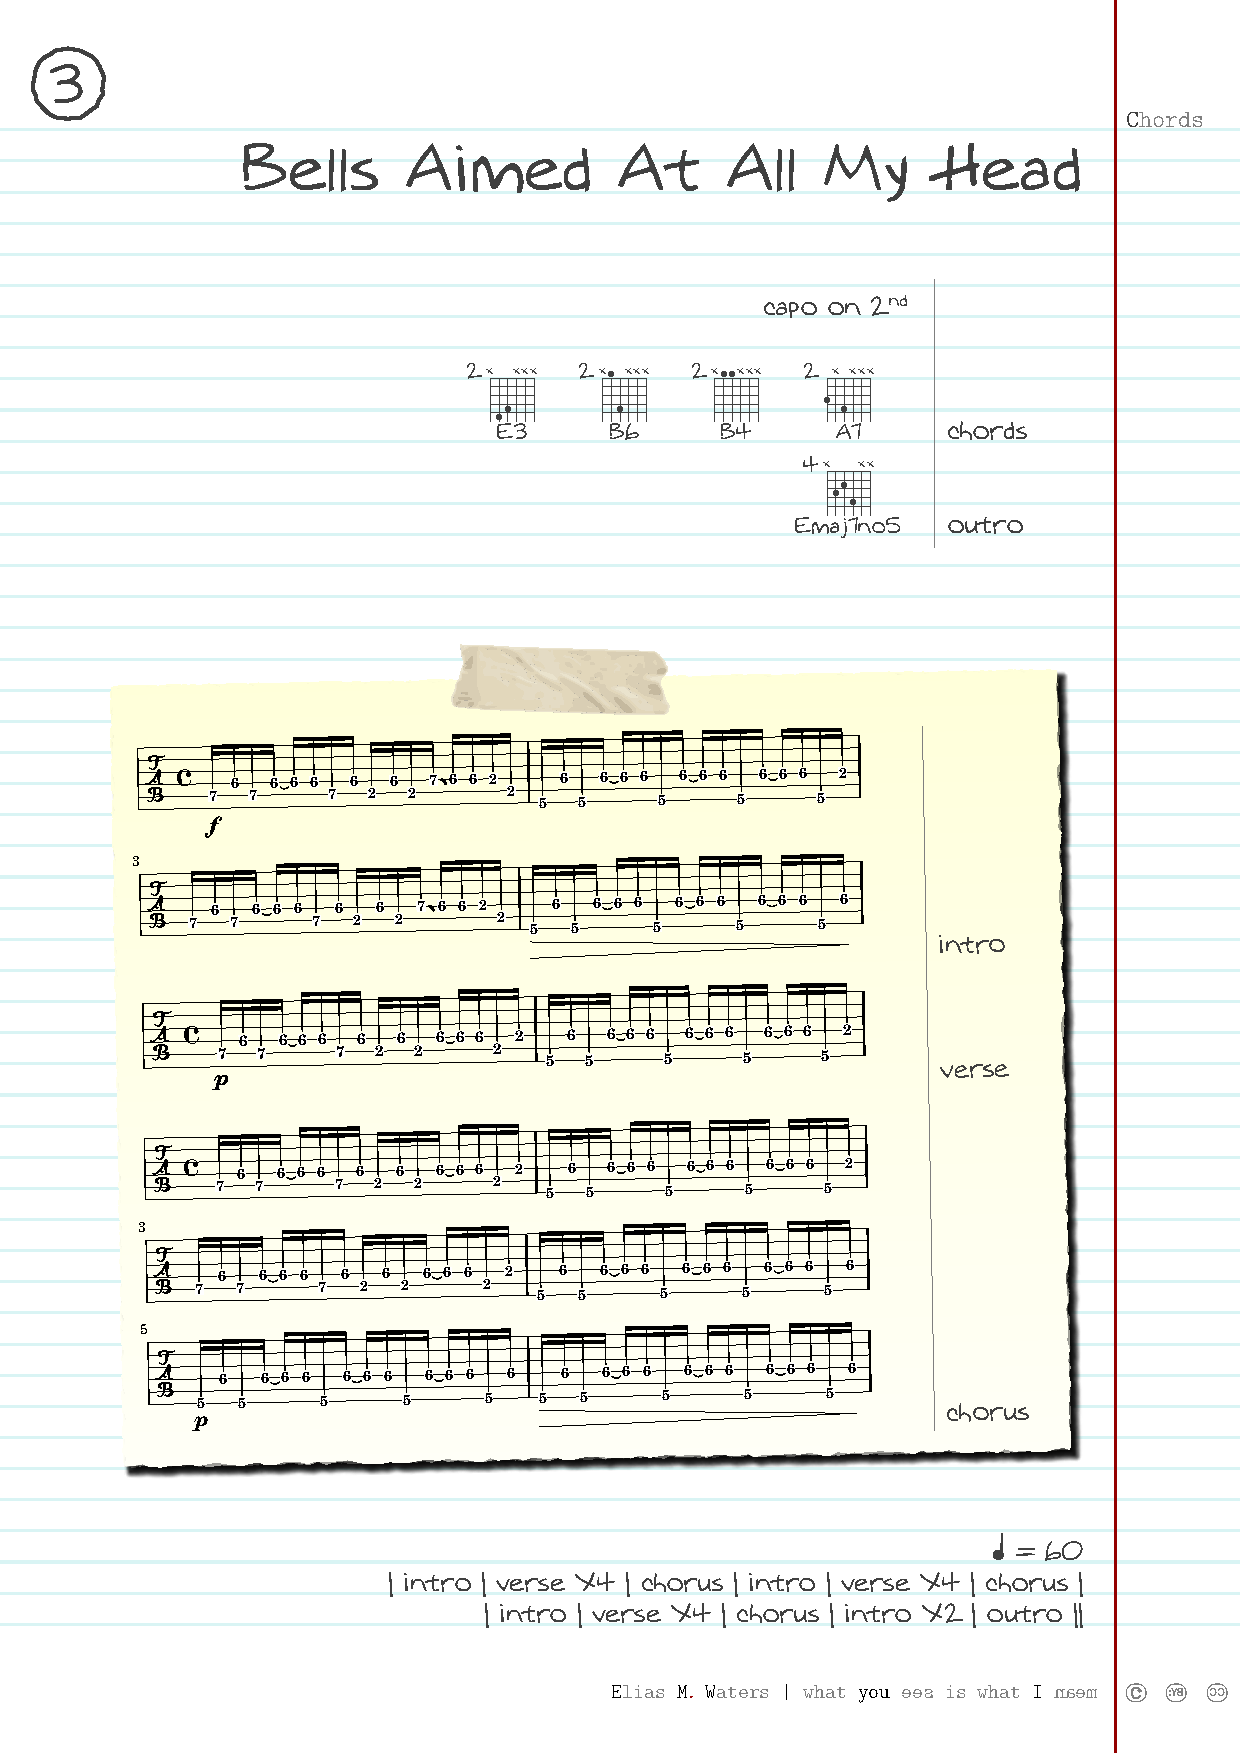
\includepdf{./FullPages/Music2.pdf}
    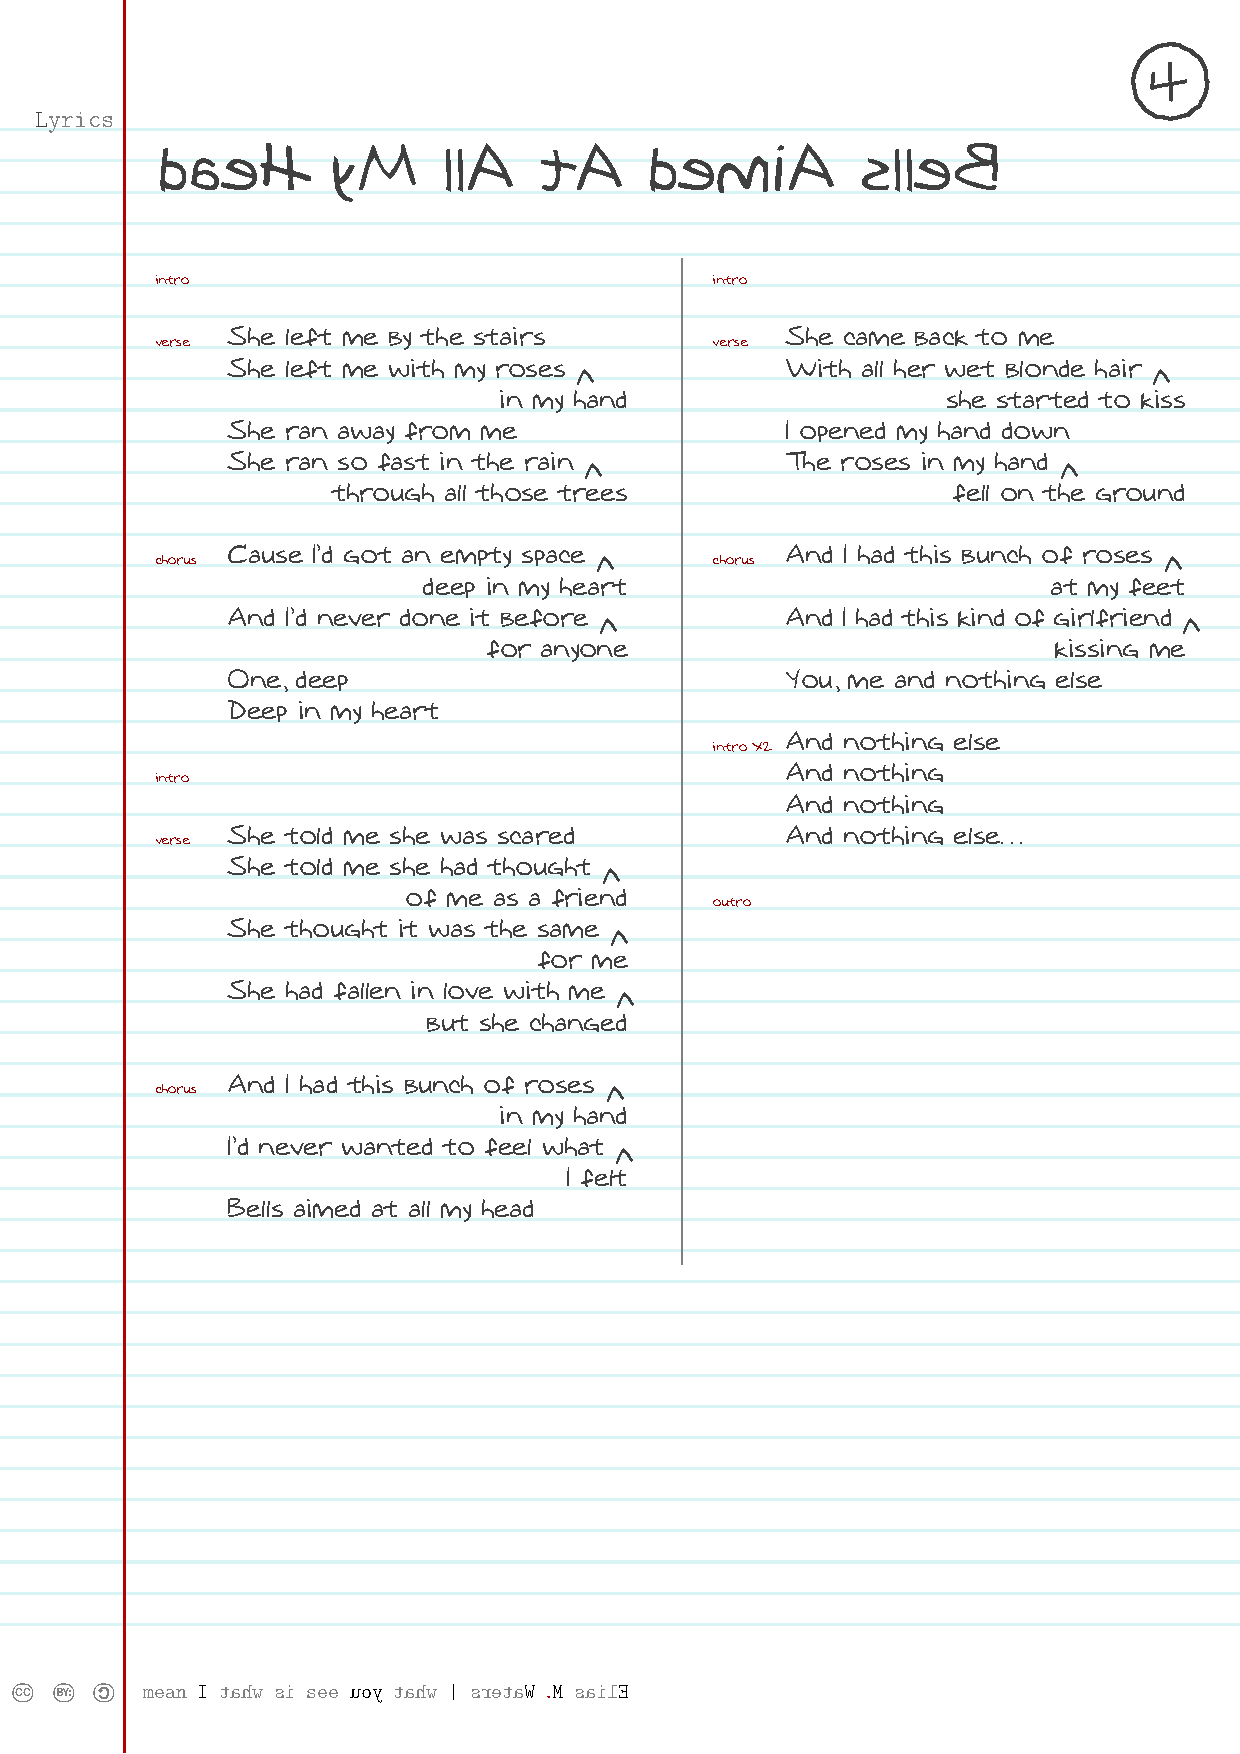
\includepdf{./FullPages/Music3.pdf}

%%%%%%%%%%%%%%%%%%%%%%%%%%%%%%%%%%%%%%%%%%%%%%%%%%%%%%%%%%%%%%%%%%%%%
% Packages
%%%%%%%%%%%%%%%%%%%%%%%%%%%%%%%%%%%%%%%%%%%%%%%%%%%%%%%%%%%%%%%%%%%%%
    \titlefleuron{Packages}{\adfoutlineleafleft}

    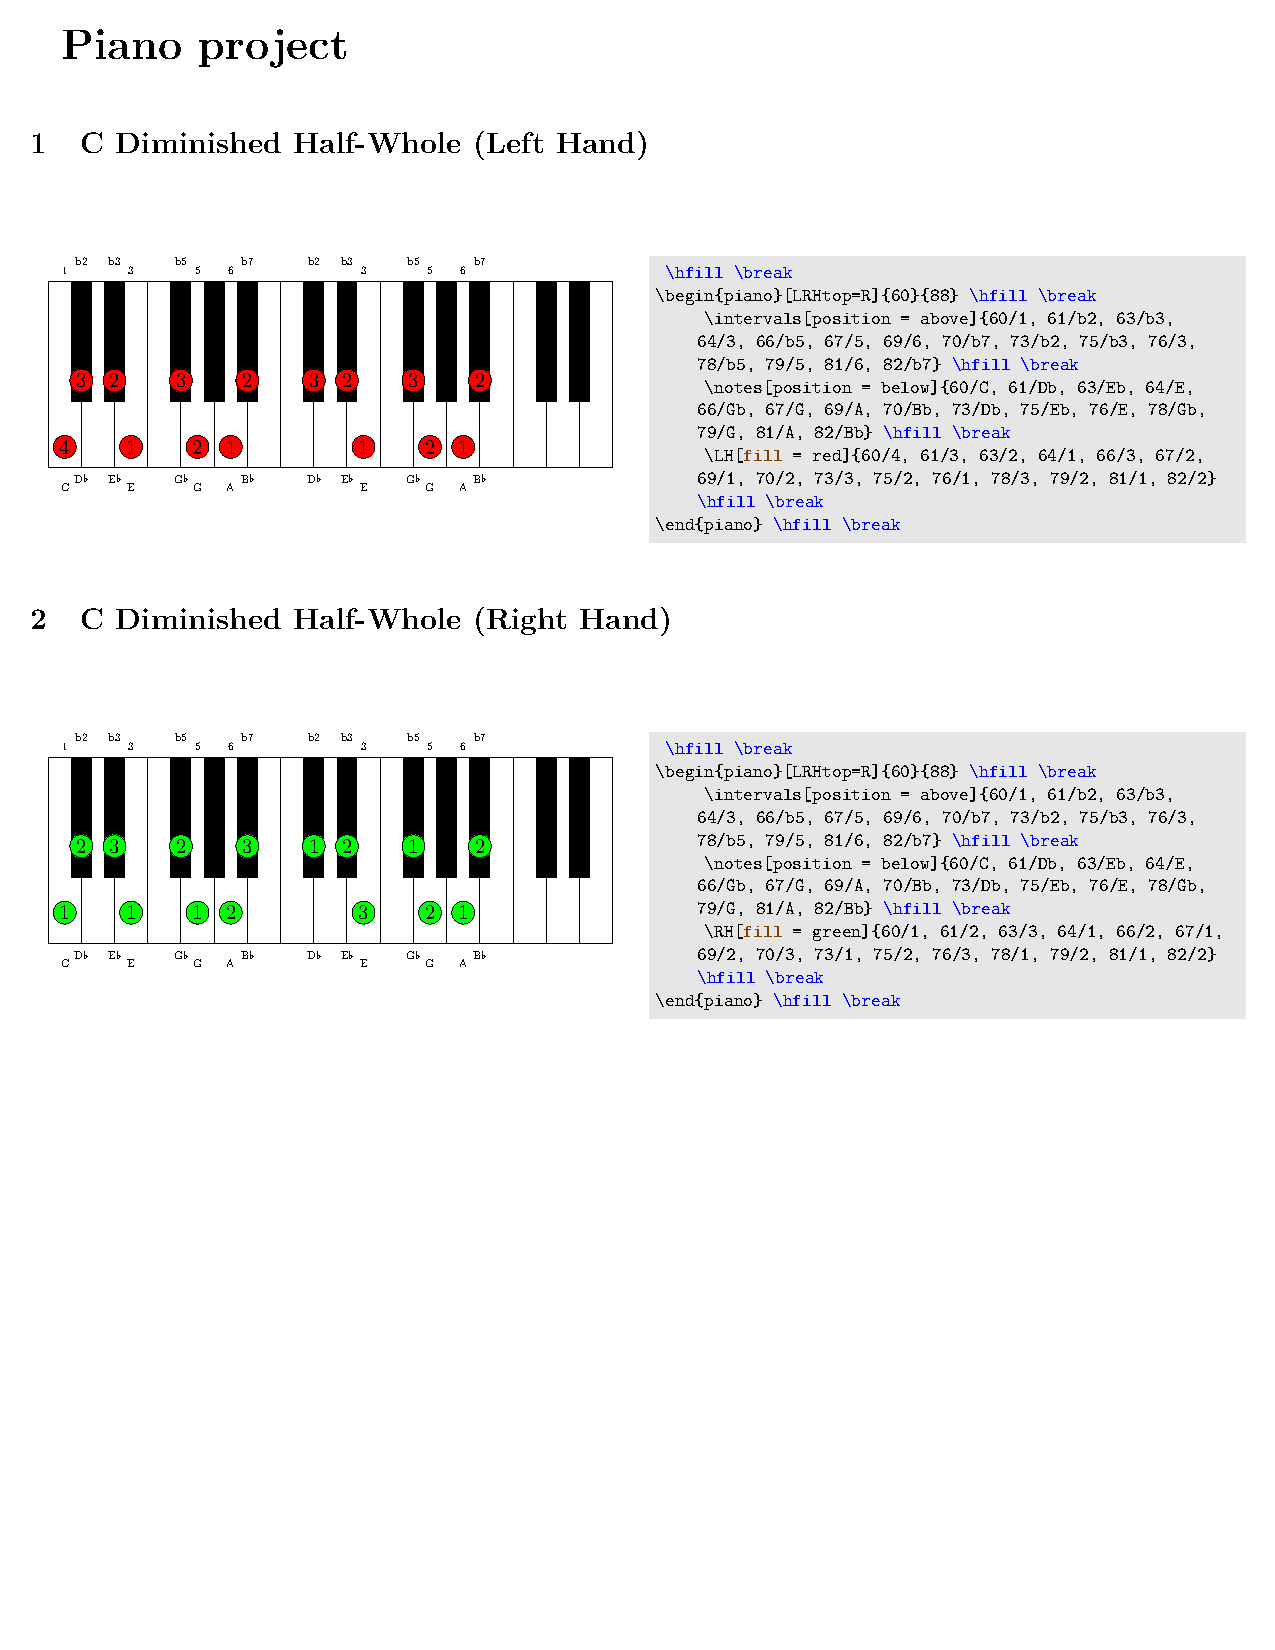
\includepdf{./FullPages/Piano1.pdf}
    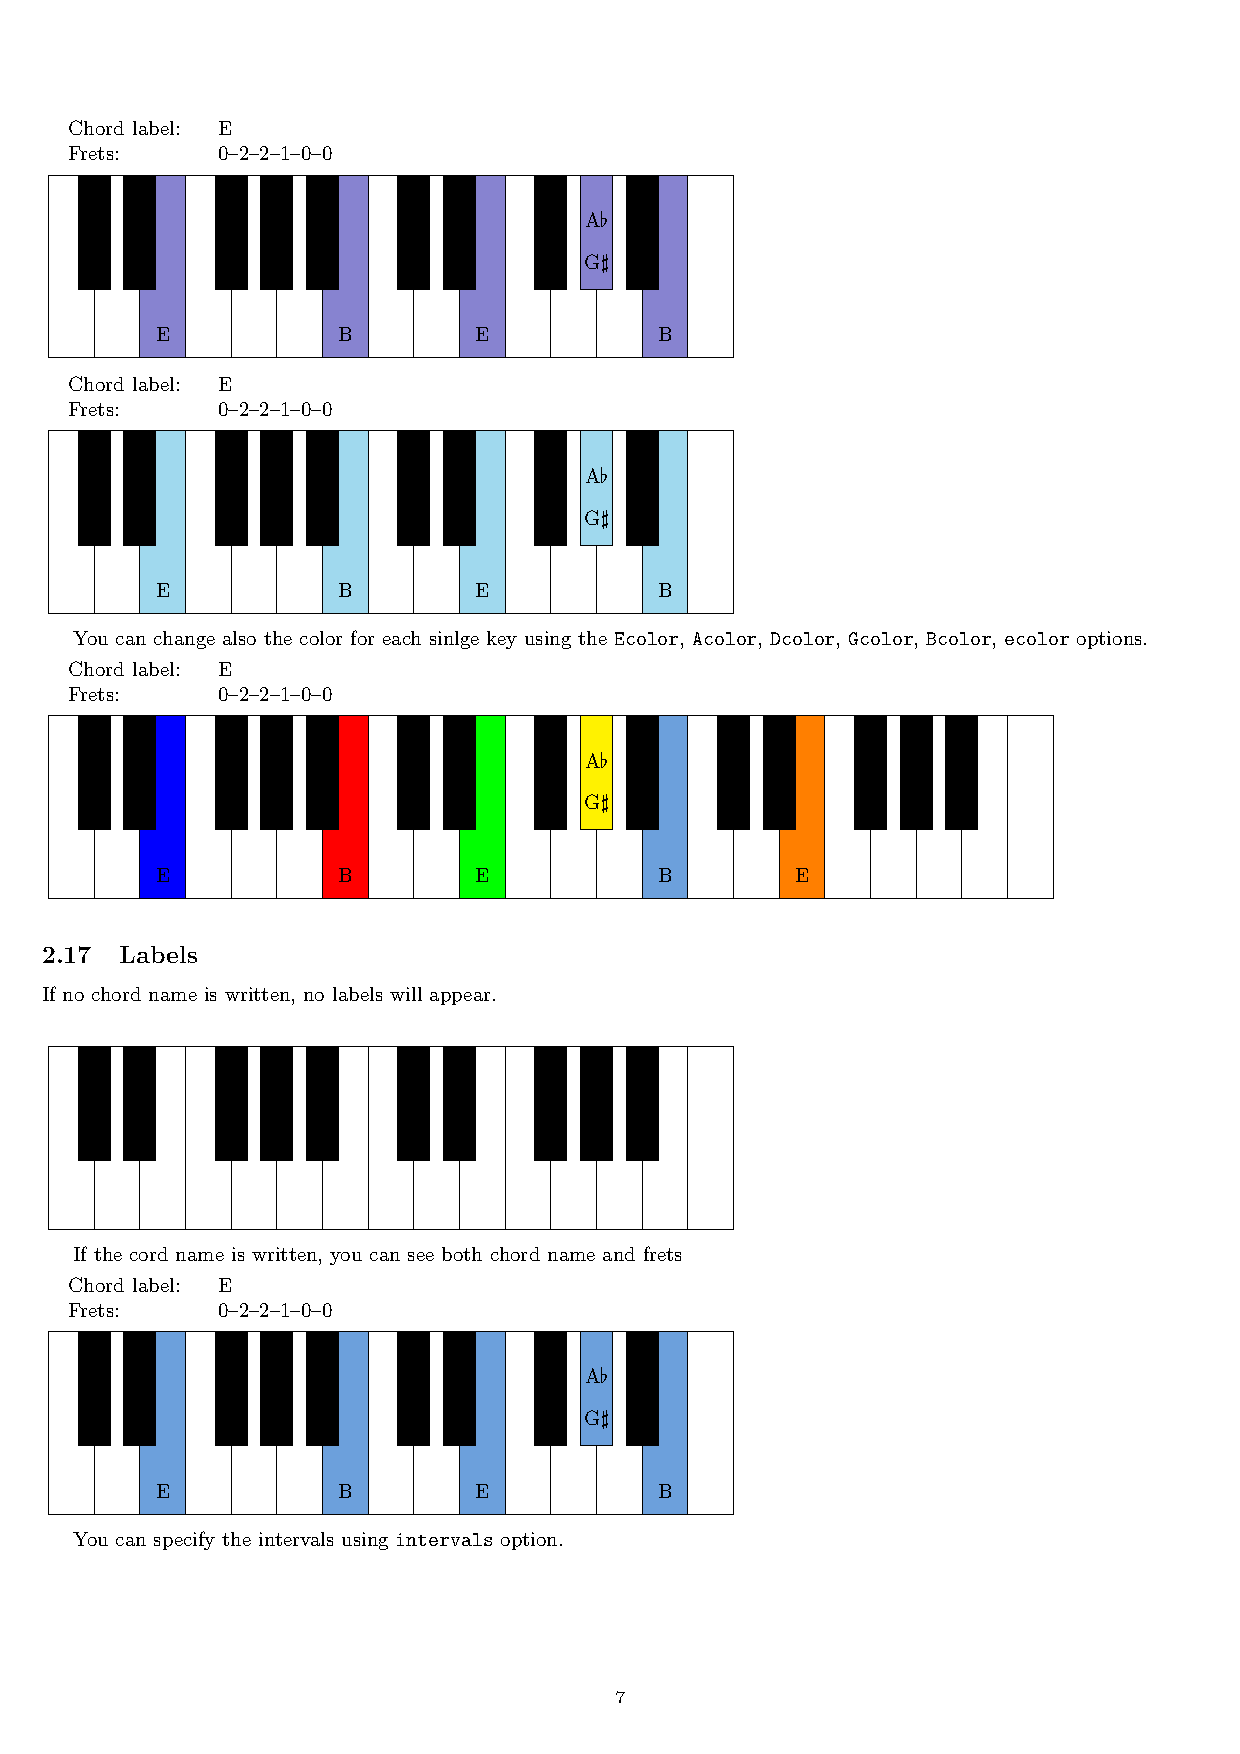
\includepdf{./FullPages/Piano2.pdf}
    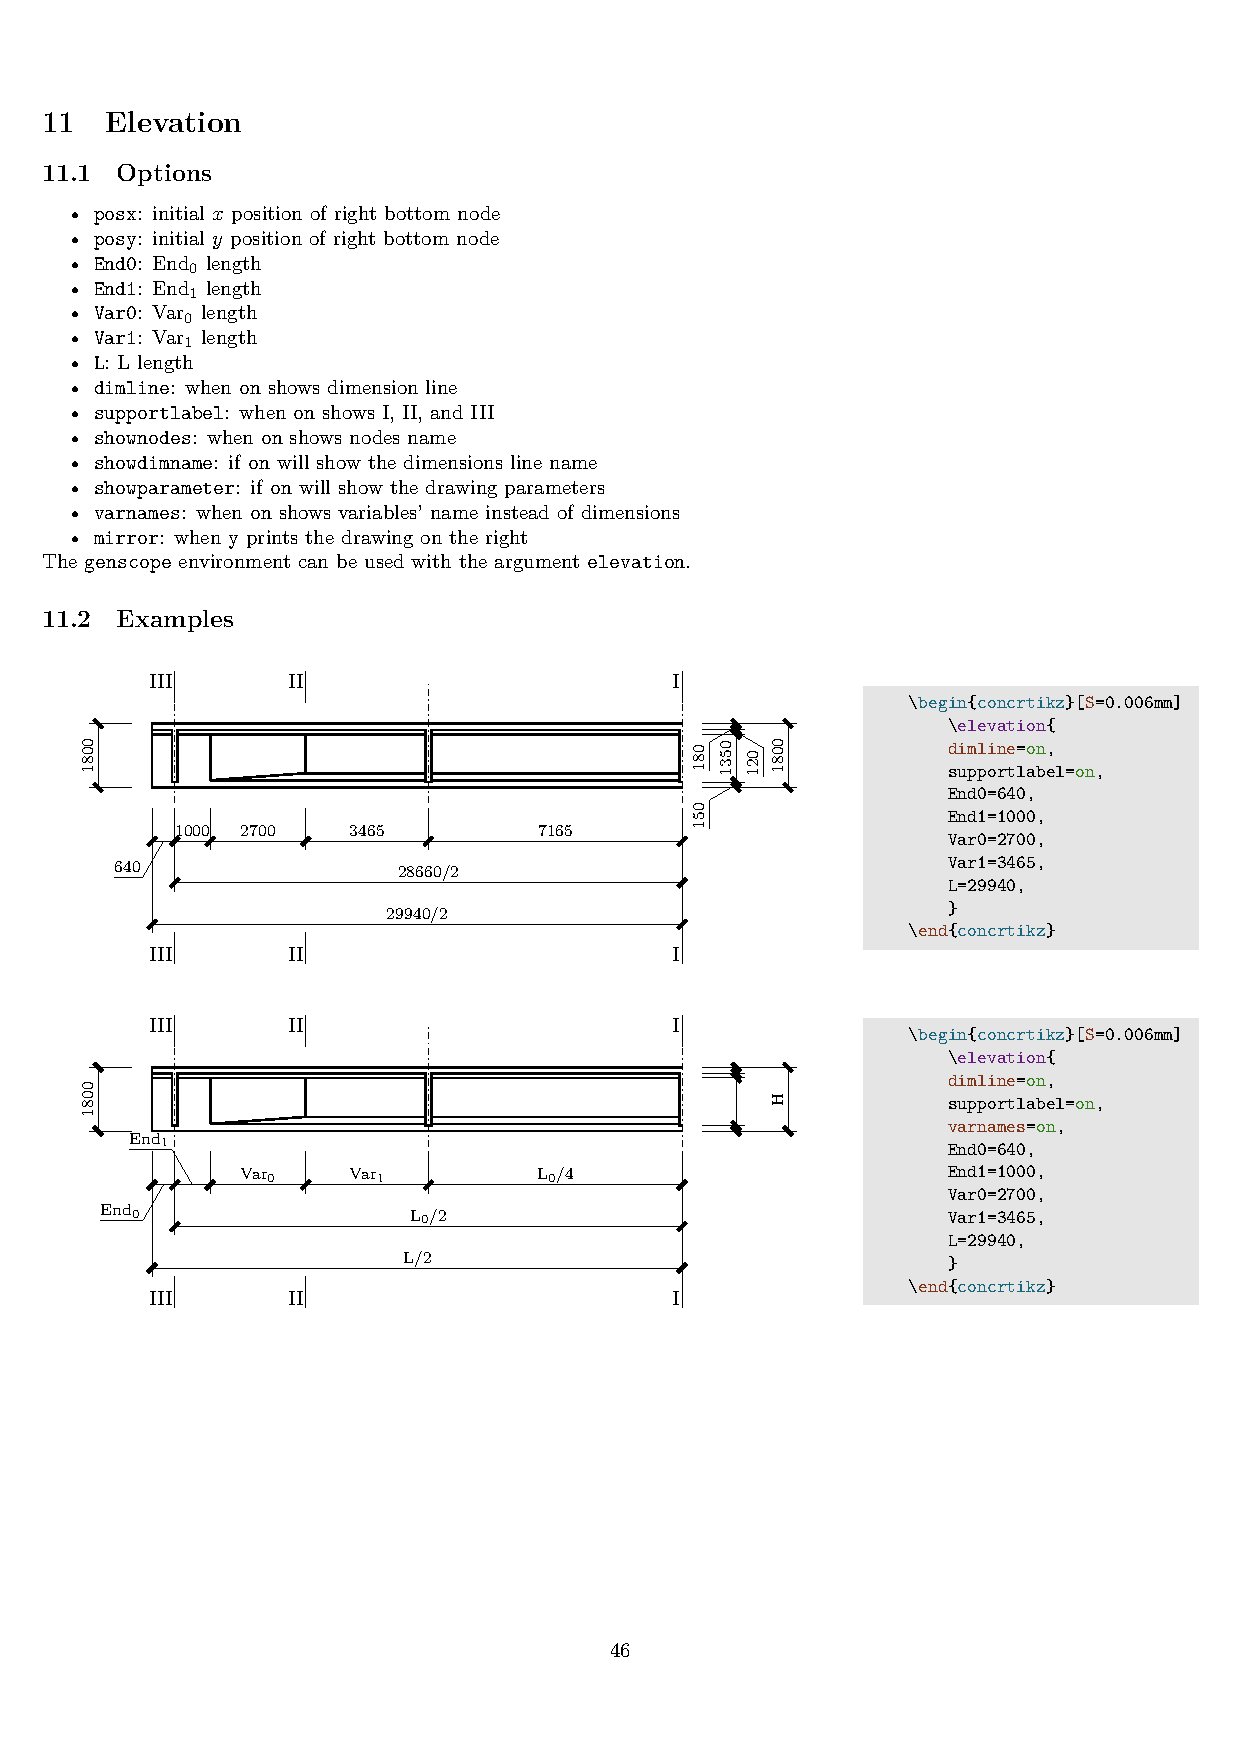
\includepdf{./FullPages/Project1.pdf}

%%%%%%%%%%%%%%%%%%%%%%%%%%%%%%%%%%%%%%%%%%%%%%%%%%%%%%%%%%%%%%%%%%%%%
% Beamer presentations
%%%%%%%%%%%%%%%%%%%%%%%%%%%%%%%%%%%%%%%%%%%%%%%%%%%%%%%%%%%%%%%%%%%%%
    \titlefleuron{Beamer presentations}{\adfflatdownhalfleafleft}

    \newgeometry{top=1cm,bottom=1cm}
    \begin{center}
        
\includegraphics[width=0.81\linewidth]{./Beamer/Page1.pdf}\\
        \vfill
        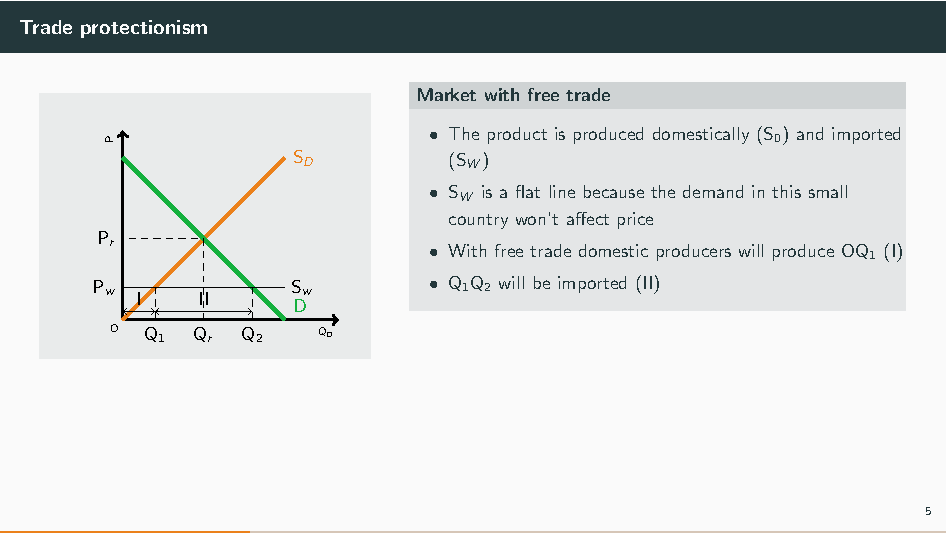
\includegraphics[width=0.81\linewidth]{./Beamer/Page2.pdf}\\
        \vfill
        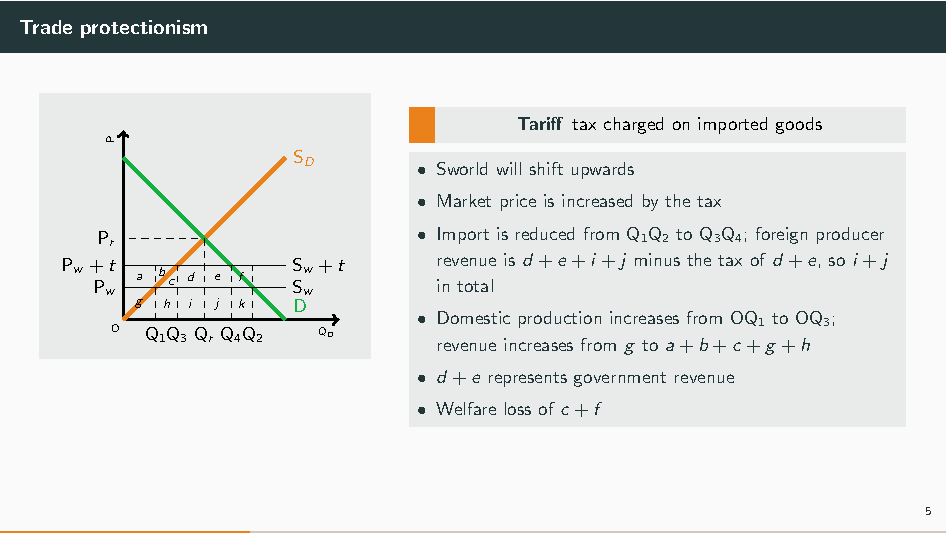
\includegraphics[width=0.81\linewidth]{./Beamer/Page3.pdf}\\
        \vfill
        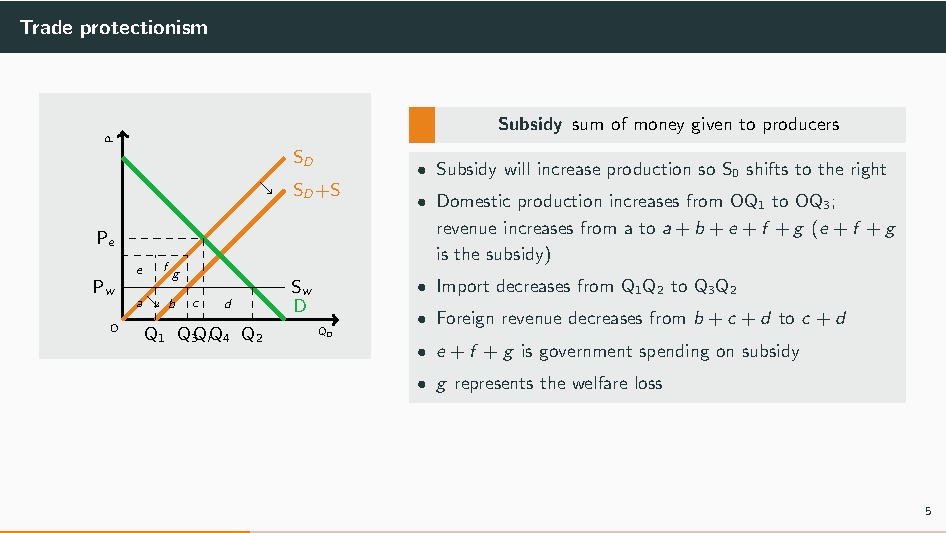
\includegraphics[width=0.81\linewidth]{./Beamer/Page4.pdf}
    \end{center}
    \clearpage
    \begin{center}
        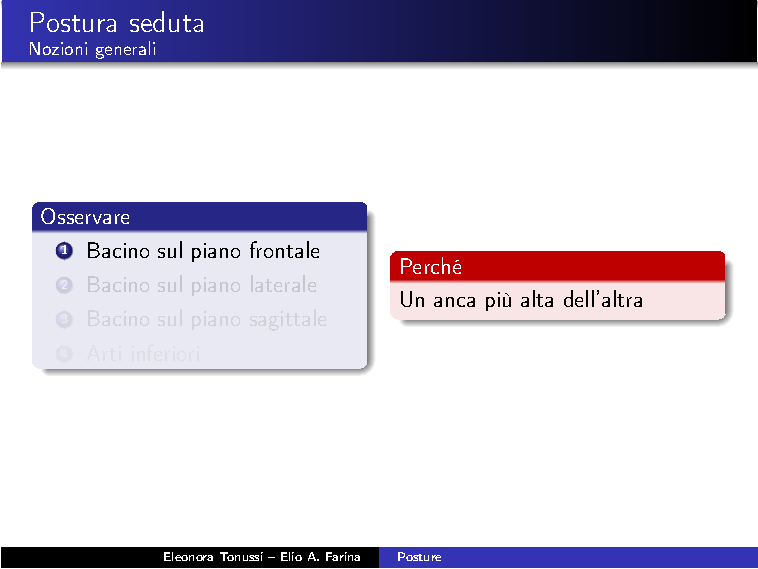
\includegraphics[width=0.81\linewidth]{./Beamer/Page6.pdf}\\
        \vfill
        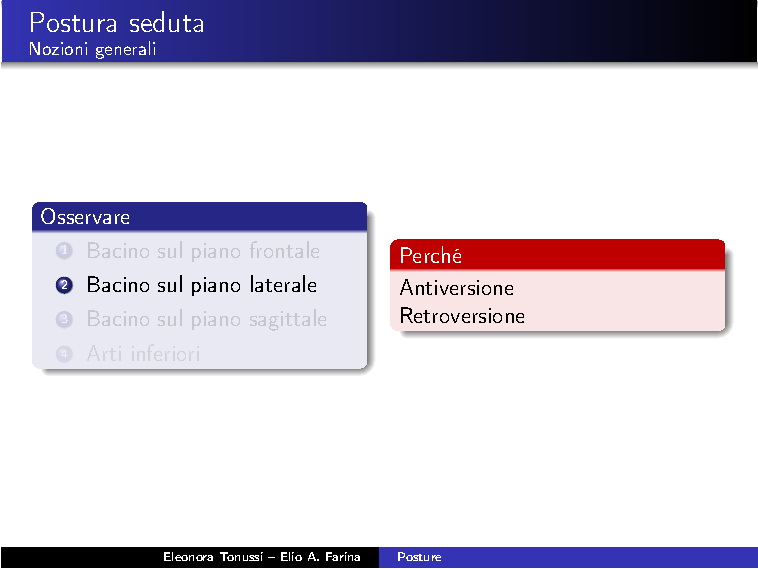
\includegraphics[width=0.81\linewidth]{./Beamer/Page7.pdf}\\
        \vfill
        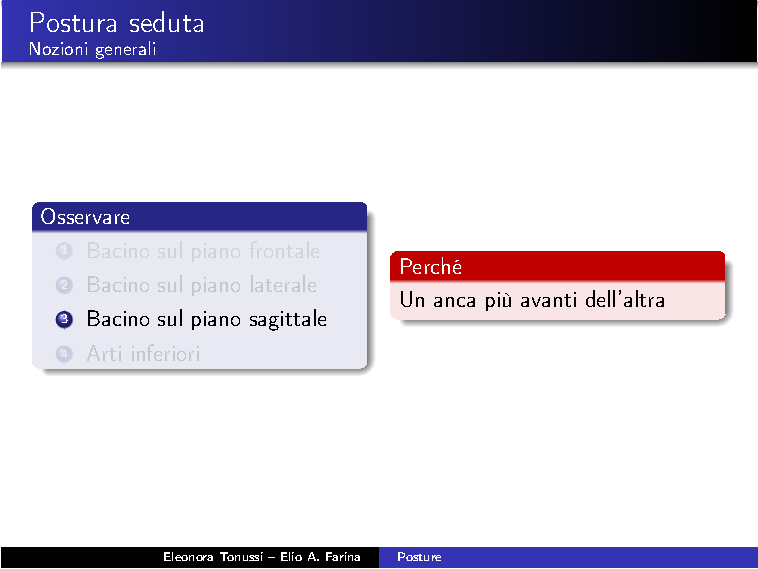
\includegraphics[width=0.81\linewidth]{./Beamer/Page8.pdf}
    \end{center}

%%%%%%%%%%%%%%%%%%%%%%%%%%%%%%%%%%%%%%%%%%%%%%%%%%%%%%%%%%%%%%%%%%%%%
% Books
%%%%%%%%%%%%%%%%%%%%%%%%%%%%%%%%%%%%%%%%%%%%%%%%%%%%%%%%%%%%%%%%%%%%%
    \restoregeometry
    \simpletitle{Printed books}

    \vfill
    \begin{minipage}{0.6\linewidth}\raggedright\Large
            \textit{A grammar of Yauyos Quechua}\\
            by Aviva Shimelman\\
            Language Science Press
        \end{minipage}\begin{minipage}{0.4\linewidth}\raggedleft
            
\includegraphics[width=\linewidth]{./FullPages/CoverAviva-crop.pdf}
    \end{minipage}

    \vfill
    \begin{minipage}{0.6\linewidth}\raggedright\Large
            \textit{Introduction to Proteins:}\\
            \textit{Structure, Function, and Motion}\\
            Second Edition\\
            by Amit Kessel and Nir Ben-Tal\\
            Chapman and Hall/CRC
        \end{minipage}\begin{minipage}{0.4\linewidth}\raggedleft
            
\includegraphics[width=\linewidth]{./FullPages/proteins}
    \end{minipage}

    \vfill
    \null

%%%%%%%%%%%%%%%%%%%%%%%%%%%%%%%%%%%%%%%%%%%%%%%%%%%%%%%%%%%%%%%%%%%%%
% Magazines
%%%%%%%%%%%%%%%%%%%%%%%%%%%%%%%%%%%%%%%%%%%%%%%%%%%%%%%%%%%%%%%%%%%%%
    \restoregeometry
    \simpletitle{Magazines and Study Guides}

    \vfill
    \begin{minipage}{0.6\linewidth}\raggedright\Large
            \textit{LED Professional Magazine}\\
            https://www.led-professional.com
        \end{minipage}\begin{minipage}{0.4\linewidth}\raggedleft
            
\includegraphics[width=\linewidth]{./FullPages/ledprofessional}
    \end{minipage}

    \vfill
    \begin{minipage}{0.6\linewidth}\raggedright\Large
            \textit{IB Academy Study Guides}\\
            https://www.ib.academy
        \end{minipage}\begin{minipage}{0.4\linewidth}\raggedleft
            
\includegraphics[width=\linewidth]{./FullPages/ibacademy}
    \end{minipage}

    \vfill
    \null

%%%%%%%%%%%%%%%%%%%%%%%%%%%%%%%%%%%%%%%%%%%%%%%%%%%%%%%%%%%%%%%%%%%%%
% Active collaborations
%%%%%%%%%%%%%%%%%%%%%%%%%%%%%%%%%%%%%%%%%%%%%%%%%%%%%%%%%%%%%%%%%%%%%
    \simpletitle{Active collaborations}

    \collaboration{IB Academy}{IBAcademylogoRed.pdf}
    \collaboration{Luger Research}{lugerlogo.jpg}
    %\collaboration{Run My Accounts}{RMAlogo.png}
    \collaboration{Silicon Prairie Portal \& Exchange}{sppxlogo.png}
    %\collaboration{Simo Publishing}{SimoLogo.pdf}

%%%%%%%%%%%%%%%%%%%%%%%%%%%%%%%%%%%%%%%%%%%%%%%%%%%%%%%%%%%%%%%%%%%%%
% Past collaborations
%%%%%%%%%%%%%%%%%%%%%%%%%%%%%%%%%%%%%%%%%%%%%%%%%%%%%%%%%%%%%%%%%%%%%
    \simpletitle{Past collaborations}

    \vspace{3\baselineskip}
    \pcollaboration{Strategic Blue}
    \begin{center}
        
\includegraphics[width=\linewidth]{./images/feedback.png}
    \end{center}

    \vspace{1\baselineskip}
    \begin{flushleft}
        \pcollaboration{Shape, BMLL, and many others\dots}
        %\pcollaboration{Active on UpWork.com and Freelancer.co.uk}
        \pcollaboration{Open to new collaboration one time only, short period, and long term}
    \end{flushleft}

    \centerfleuron{\adfdownleafleft}

%%%%%%%%%%%%%%%%%%%%%%%%%%%%%%%%%%%%%%%%%%%%%%%%%%%%%%%%%%%%%%%%%%%%%
% Type of collaborations
%%%%%%%%%%%%%%%%%%%%%%%%%%%%%%%%%%%%%%%%%%%%%%%%%%%%%%%%%%%%%%%%%%%%%
    \simpletitle{Type of collaborations}

    \vspace{3\baselineskip}
    \begin{flushleft}
        \pcollaboration{Help with thesis, master thesis, documents, CV, \dots}
        \pcollaboration{IEEE and other template adaptations}
        \pcollaboration{Book publishing adaptations}
        \pcollaboration{Conversion from MSWord (.doc) to \LaTeXe\ (.tex)}
        \pcollaboration{Bib\TeX\ research and coding}
        \pcollaboration{TikZ graphs, diagrams, flowcharts, and design}
        \pcollaboration{Template (class) creation}
        \pcollaboration{Packages creation}
        \pcollaboration{Document layout}
        \pcollaboration{Document creation}
        \pcollaboration{Document and report creation from database entries}
        \pcollaboration{Beamer presentations}
        \pcollaboration{\tt pdflatex/xelatex}
        \pcollaboration{Account on Overleaf, GitHub, and BitBucket}
    \end{flushleft}

    \centerfleuron{\adfflatleafsolidleft}

%%%%%%%%%%%%%%%%%%%%%%%%%%%%%%%%%%%%%%%%%%%%%%%%%%%%%%%%%%%%%%%%%%%%%
% Feedbacks
%%%%%%%%%%%%%%%%%%%%%%%%%%%%%%%%%%%%%%%%%%%%%%%%%%%%%%%%%%%%%%%%%%%%%
    \simpletitle{A collection of feedback*}

    \vfill
    \begin{center}\LARGE\tt
        Rule \#1:\\
        Use whatever Elio recommends.\\
        \strut\\
        Rule \#2:\\
        Don't forget rule \#1.\\
        \strut\\
        \large Blaise Pabon
    \end{center}
    \vfill
    * From personal messages, LinkedIn, UpWork.com and Freelancer.co.uk transcribed \texttt{verbatim}

    \clearpage
    \newgeometry{top=3cm,bottom=3cm}
    \feedback[\huge]{Great help from Elio! I will surely ask him for help again.}
\feedback{Was an absolute pleasure to work with Elio. He was extremely professional and knows his stuff. Would highly recommend him.}
\feedback{Elio completed the conversion of a technical document from word to LaTeX. He completed the work extremely efficiently, and I was very pleased at all the extra suggestions he made and completed to make the document look as professional as possible. I highly recommend Elio and would have no hesitation in working with him again.}
\feedback{Working with Elio was a very pleasant experience and I can highly recommend him for any LaTeX typesetting challenges and complex TikZ drawings. My project had a very tight deadline and he delivered on time and provided me with a great result. Great communication throughout the duration of the project.
I will work with him again.}
\feedback{Elio's great! Highly recommend. Thoughtful, prompt, and skilled!}
\feedback[\huge]{He is a Latex Jedi.}
\feedback{Elio was great to work with. He is very knowledgeable about LaTeX, gave a quality product, was friendly, and was very fast in completing the task. I would definitely work with him again or recommend him to my friends and colleagues.}
\feedback{Best Latex expert with a great communication skills. I highly recommend him and I will keep using him.
Thank you so much for the best latex edit.}
\feedback{A wonderful latex expert! He did not just complete the work successfully but also answer my questions patiently. I highly recommend him.}
\feedback[\huge]{Elio was really great to work with. He is a true LaTeX expert! Highly recommended.}
%%%%%%%%%%%%%%%%%%%%%%%%%%%%%%%%%%%%%%%%%%%%%%%%%%%%%%%%%%%%%%%%%%%%%
\feedback[\huge]{I've said it again and will say again. Will keep working with Elio. Awesome for LaTex}
\feedback{Elio is excellent with LaTeX and really blends functionality with design. We were on a tight deadline, his communication was of a very high standard and we have no hesitation in recommending him. Thank you for a really well delivered project. I hope we can work with you again soon.}
\feedback{Working with Elio has helped me in so many ways: Elio is clever and has an intimate knowledge of LaTeX, he has attention for detail and a feeling for what looks good, he is able to solve problems before they even come to your attention. Elio loves LaTeX.\\
He is also funny, easy to talk to and overall a great guy - just a pleasure.\\
Finally, he's worked mostly manual hours (not time logged in the work diary) and he has always logged very modest amounts of hours. Elio is extremely reliable and will never overcharge, if anything he undercharges.\\
He's been the best freelancer experience that I have had, and I will continue to work with Elio for a long time!}
\feedback[\huge]{Thank you Elio.}
\feedback{I needed Elio's expertise in Latex for converting a bunch of lyx file into dissertation latex with strict template. I had many big tables and Elio was able to change all of them nicely to fit within the margins.\\
Since this was an important job, I hired 2 other upwork workers besides Elio. The other two weren't able to deliver what I needed. Elio delivered what I needed in less than half the time the other people took and delivered 100\%! Where other two highly rated latex experts failed, Elio succeeded.\\
He really cares a lot about the work. THE BEST UPWORK person I've ever worked with!\\
HIRE THIS GUY!}
\feedback{Elio is the most thorough, meticulous and pleasant consultant I have worked with during my twenty-six years in the IT business. His work is of astonishing quality, exceeding my most ambitious expectations.}
%%%%%%%%%%%%%%%%%%%%%%%%%%%%%%%%%%%%%%%%%%%%%%%%%%%%%%%%%%%%%%%%%%%%%
\feedback[\huge]{It's not standard to work with such experts}
\feedback{Excellent work! Accurate, fast and even took initiative to make improvements not included on the original task. I am very happy to find someone who is genuinely interested in the quality of their work. Will certainly use again. Thank you.}
\feedback{Fantastic project!}
\feedback{Elio was excellent; he created a TikZ image based on a .png I sent him. I needed a few versions (i.e. with different elements selected). Elio implemented this as two function calls, one to plot and one to highlight, that allowed me to make minor adjustments (i.e. to the color scheme) to all of the figures at once (i.e. by tweaking parameters in the function) as I've further iterated on the slide deck. Furthermore, I posted this request on my way out of the office in the hopes of having a solution before the morning. Elio had the deliverable in my inbox within an hour. 10/10.}
\feedback{Great help from Elio! I will surely ask him for help again.}
\feedback{Elio was great to work with. He is very skilled in LateX, and he also had the right musical knowledge to help me with formatting my book with piano diagrams. I'd hire him again.}
\feedback{Elio is extremely helpful and the results of his work are very good.}
\feedback[\huge]{Was an absolute pleasure to work with Elio. He was extremely professional and knows his stuff. Would highly recommend him.}
%%%%%%%%%%%%%%%%%%%%%%%%%%%%%%%%%%%%%%%%%%%%%%%%%%%%%%%%%%%%%%%%%%%%%
\clearpage
\feedback[\huge]{Elio is fantastic, competent and really does all he can to get the result I want}

\feedback{Fast delivery on Latex TIKZ project.}

\feedback{Elio was once again fantastic. He is a real pleasure to work with and very communicative, and will always offer helpful suggestions for project improvement beyond what I expected! A*}

\feedback{100\% amazing. 5 stars. ***** Elio was very communicative and very easy to talk to about the project. He put in a lot of time and went above and beyond what I expected. He offered advice on the content of my work and this was very helpful, even thought this was not part of the work I expected him to do. He was able to accommodate my needs and asking him to make changes when I changed my mind on something was very easy. I am already certain that I will be using Elio again in the future for my work and I would highly recommend other people hire him. Also, it was nice to get to know Elio as he is a very nice person.}

\feedback[\huge]{Elio did everything I asked and more. My original brief changed a couple of times through the project and Elio evolved with the project and made sure my vision was realised.}


%%%%%%%%%%%%%%%%%%%%%%%%%%%%%%%%%%%%%%%%%%%%%%%%%%%%%%%%%%%%%%%%%%%%%
% Last page
%%%%%%%%%%%%%%%%%%%%%%%%%%%%%%%%%%%%%%%%%%%%%%%%%%%%%%%%%%%%%%%%%%%%%
    \clearpage
    \null
    \vfill
    \begin{center}
    \includegraphics[width=0.6\linewidth]{./TikZimages/logotest.pdf}
    \end{center}
    \vfill
    \null

\end{document}